% =====================================================================
%  TRABAJO FIN DE MÁSTER
%  Máster en Data Science, Big Data & Business Analytics — UCM
%  Autora: Keyla Lisbeth López Chamorro
%
%  NOTA SOBRE EL FORMATO
%  La guía del TFM prohíbe expresamente el formato de artículo científico.
%  Este documento se estructura como INFORME TÉCNICO ORIENTADO A NEGOCIO:
%  sin abstract, sin keywords y sin sección de "trabajos relacionados".
%
%  TRAZABILIDAD DE LAS CIFRAS
%  Todos los números provienen de resultados/metricas/*.json, generados por
%  una ejecución real del código. No hay ninguna cifra estimada.
%
%  Compilar:  pdflatex memoria.tex   (dos veces, para el índice)
% =====================================================================
\documentclass[11pt,a4paper]{article}

\usepackage[utf8]{inputenc}
\usepackage[T1]{fontenc}

\IfFileExists{spanish.ldf}%
  {\usepackage[spanish,es-tabla,es-noquoting]{babel}}%
  {\usepackage[english]{babel}}

\usepackage{amsmath}

% Tipografía por defecto de LaTeX (Computer Modern), de aspecto académico
% clásico. NOTA: la guía del TFM recomienda Verdana o Arial. Si prefieres
% seguir esa recomendación, descomenta las dos líneas siguientes.
% \usepackage{helvet}
% \renewcommand{\familydefault}{\sfdefault}

\usepackage[margin=2.5cm]{geometry}
\usepackage{graphicx}
\usepackage{booktabs}
\usepackage{xcolor}
\usepackage{caption}
\usepackage{enumitem}
\usepackage{fancyhdr}
\usepackage{tocloft}   % control fino del índice
% Índice algo más compacto, para que quepa entero en una sola página.
\setlength{\cftbeforesecskip}{0.45ex}
\setlength{\cftbeforesubsecskip}{0.15ex}
\usepackage[hidelinks]{hyperref}

\graphicspath{{../resultados/figuras/}}
\captionsetup{font=small,labelfont=bf}
\setlength{\parskip}{0.55em}
\setlength{\parindent}{0pt}
\linespread{1.06}

% Evita líneas viudas y huérfanas: impide que la última línea de un párrafo
% quede sola al principio de una página (o la primera al final de la anterior).
\widowpenalty=10000
\clubpenalty=10000
\displaywidowpenalty=10000

\definecolor{azulucm}{RGB}{0,45,98}
\definecolor{azulclaro}{RGB}{0,120,190}
\pagestyle{fancy}\fancyhf{}
\rhead{\small\textcolor{gray}{TFM — Inteligencia de reseñas de pacientes}}
\rfoot{\small\thepage}
\renewcommand{\headrulewidth}{0.2pt}

% Recuadro para los mensajes dirigidos a negocio. En tono neutro, para
% mantener la coherencia con el resto del documento.
\newcommand{\ideaclave}[1]{%
  \begin{center}\fcolorbox{black!45}{black!4}{%
  \parbox{0.94\textwidth}{\small\textbf{Idea clave.} #1}}\end{center}}

\newcommand{\autortfm}{Keyla Lisbeth López Chamorro}

\begin{document}

% Rótulos en español fijados a mano. Deben ir DESPUÉS de \begin{document}:
% babel reescribe estos nombres al iniciar el documento, de modo que si se
% definen en el preámbulo quedan sobrescritos. Con esto el documento sale en
% español aunque la distribución de LaTeX no tenga babel-spanish instalado
% (paquete texlive-lang-spanish), que es lo que provocaría ver "Figure",
% "Table", "References" o "Contents" en inglés.
\renewcommand{\figurename}{Figura}
\renewcommand{\tablename}{Tabla}
\renewcommand{\refname}{Referencias}
\renewcommand{\contentsname}{Índice}
\renewcommand{\appendixname}{Anexo}

% =====================================================================
\begin{titlepage}
\thispagestyle{empty}
\centering

\vspace*{1.5cm}

{\large Universidad Complutense de Madrid\par}
\vspace{0.35cm}
{\large Facultad de Comercio y Turismo\par}

\vspace{1.8cm}

{\normalsize Máster de Formación Permanente en\par}
\vspace{0.3cm}
{\large\scshape Data Science, Big Data \& Business Analytics\par}

\vspace{3.2cm}

\rule{\textwidth}{0.4pt}
\vspace{0.7cm}

{\LARGE\bfseries Inteligencia de reseñas de pacientes\par}

\vspace{0.7cm}

{\large Análisis de sentimiento y descubrimiento de temas\\
mediante NLP, con despliegue de un modelo productivizable\par}

\vspace{0.7cm}
\rule{\textwidth}{0.4pt}

\vspace{2.2cm}

{\large Trabajo Fin de Máster\par}

\vspace{2.2cm}

{\large
\begin{tabular}{@{}r@{\hspace{0.8em}}l@{}}
  Autora:  & \autortfm \\[0.3cm]
  Tutores: & Carlos Ortega y Santiago Mota \\
\end{tabular}\par}

\vfill

{\large Septiembre de 2026\par}
\vspace{1cm}
\end{titlepage}

\tableofcontents
\newpage

% =====================================================================
\section{Resumen ejecutivo}
% =====================================================================

Las plataformas de salud acumulan millones de opiniones escritas por pacientes
que hoy apenas se explotan. Dentro de ese texto libre hay información sobre
qué medicamentos funcionan, cuáles generan efectos adversos y qué preocupa
realmente a quien los toma. Leer ese volumen de forma manual es inviable.

Este trabajo convierte ese texto en información accionable. Partiendo de
\textbf{213.807 reseñas reales} de pacientes sobre \textbf{3.658 medicamentos}
y \textbf{836 condiciones médicas}, se ha construido un sistema capaz de:

\begin{enumerate}[nosep,leftmargin=*]
  \item clasificar automáticamente si una opinión es favorable o desfavorable;
  \item descubrir de qué hablan los pacientes (eficacia, efectos secundarios,
        posología, coste) sin definir esas categorías de antemano;
  \item explicar en qué se ha basado cada decisión concreta.
\end{enumerate}

El modelo seleccionado, una \textbf{máquina de vectores de soporte lineal},
alcanza un \textbf{F1 de 0,9494} y un \textbf{ROC-AUC de 0,9649} evaluado sobre
\textbf{721 medicamentos que nunca aparecieron durante el entrenamiento}. Esta
condición de evaluación es deliberadamente exigente y se justifica en la
sección~\ref{sec:particion}.

El modelo se ha empaquetado en una aplicación que recibe una reseña nueva y
devuelve, en tiempo real, la predicción, los aspectos detectados y los términos
que han pesado en la decisión.

\ideaclave{El sistema permite detectar señales negativas sobre un medicamento
sin leer manualmente miles de reseñas. Sobre las 213.807 opiniones analizadas,
identifica automáticamente las 53.235 desfavorables y explica por qué lo son,
reduciendo drásticamente el tiempo de reacción en farmacovigilancia.}

% =====================================================================
\section{Introducción y contexto de negocio}
% =====================================================================

\subsection{El problema}

Cuando un paciente abandona un tratamiento, rara vez lo comunica a su médico:
lo escribe en internet. Esa información existe, es pública y está sin explotar.

Las áreas de farmacovigilancia trabajan hoy con notificaciones formales de
reacciones adversas, un canal fiable pero lento e infrautilizado. Las reseñas
de pacientes ofrecen una señal complementaria: masiva, inmediata y espontánea.
Su inconveniente es el formato —texto libre, sin estructura, con faltas de
ortografía y jerga— que impide analizarlas con herramientas convencionales.

El coste de no hacerlo es doble. Por un lado, se pierde tiempo de reacción ante
un problema de seguridad. Por otro, se desconoce qué mueve realmente la
satisfacción del paciente, información valiosa para decidir sobre un
tratamiento o priorizar la comunicación con el usuario.

\subsection{Objetivos}

\begin{enumerate}[nosep,leftmargin=*]
  \item \textbf{Clasificar} automáticamente el sentimiento de una reseña.
  \item \textbf{Descubrir} los temas y aspectos predominantes en el corpus.
  \item \textbf{Explicar} las predicciones de forma comprensible para negocio.
  \item \textbf{Desplegar} el modelo en una aplicación que acepte reseñas nuevas.
\end{enumerate}

\subsection{Preguntas de investigación}

\begin{itemize}[nosep,leftmargin=*]
  \item[\textbf{P1}] ¿Puede predecirse la satisfacción del paciente únicamente
        a partir del texto que escribe?
  \item[\textbf{P2}] ¿Generaliza el modelo a medicamentos que nunca ha visto?
  \item[\textbf{P3}] ¿Qué aspectos concentran la insatisfacción, y coinciden
        con los que cabría esperar?
\end{itemize}

La sección~\ref{sec:aspectos} muestra que la respuesta a P3 es contraintuitiva.

% =====================================================================
\section{El conjunto de datos}
% =====================================================================

\subsection{Fuente, licencia y derechos de uso}

Se emplea el \textit{Drug Review Dataset} (Drugs.com), publicado en el UCI
Machine Learning Repository (DOI 10.24432/C5SK5S) bajo licencia CC BY 4.0. Los
autores autorizan su uso con fines de investigación, sin explotación comercial
ni redistribución, y con cita del trabajo original~\cite{graesser2018}.
El uso realizado en este TFM cumple íntegramente esas condiciones.

\subsection{Estructura y volumen}

\begin{table}[htbp]\centering\small
\caption{Variables del conjunto de datos.}
\begin{tabular}{@{}lll@{}}
\toprule
\textbf{Variable} & \textbf{Tipo} & \textbf{Descripción} \\ \midrule
\texttt{drugName}    & Categórica & Nombre del medicamento (3.658 distintos) \\
\texttt{condition}   & Categórica & Condición médica tratada (836 distintas) \\
\texttt{review}      & Texto      & Opinión libre del paciente \\
\texttt{rating}      & Numérica   & Valoración de 1 a 10 \\
\texttt{date}        & Fecha      & Publicación, de feb.~2008 a dic.~2017 \\
\texttt{usefulCount} & Numérica   & Usuarios que la marcaron como útil \\ \bottomrule
\end{tabular}
\end{table}

La longitud media de una reseña es de \textbf{84,7 palabras} (445,8 caracteres),
suficiente para aplicar técnicas de NLP con garantías.

\subsection{Calidad de los datos y limpieza aplicada}

El fichero original presenta tres problemas que, de no corregirse,
comprometerían el análisis. Se documentan aquí porque el diagnóstico de la
calidad del dato es parte del trabajo, no un trámite previo.

\begin{enumerate}[leftmargin=*]
  \item \textbf{Codificación HTML doble.} Los apóstrofos aparecen como
        \texttt{\&\#039;} y las reseñas van envueltas en comillas duplicadas.
        Sin corregirlo, la tokenización fragmenta palabras como
        \textit{don't} en unidades sin sentido.
  \item \textbf{Filas corruptas.} \textbf{1.171 registros} contienen, en el
        campo \texttt{condition}, fragmentos de HTML procedentes del proceso
        de extracción original (por ejemplo,
        \texttt{"3</span> users found this comment helpful"}). Se eliminan.
  \item \textbf{Duplicados exactos.} Se detectan y eliminan \textbf{85 reseñas}
        idénticas en texto, medicamento y condición. Aunque son pocas, su
        eliminación es imprescindible: una reseña repetida a ambos lados de la
        partición produciría fuga de información y métricas artificialmente
        optimistas.
\end{enumerate}

Tras la limpieza se conservan \textbf{213.807 reseñas} de las 215.063
originales. Persisten 1.194 registros sin condición asignada, que se mantienen
por ser válidos para el análisis de texto.

\subsection{Limitaciones y consideraciones éticas}

\begin{itemize}[nosep,leftmargin=*]
  \item \textbf{Sesgo de autoselección.} Quien escribe una reseña no es un
        paciente medio: suele hacerlo cuando el resultado ha sido muy bueno o
        muy malo. La sección~\ref{sec:eda} lo confirma empíricamente.
  \item \textbf{Ausencia de verificación clínica.} No hay diagnóstico
        confirmado ni seguimiento médico detrás de cada texto.
  \item \textbf{Privacidad.} Las reseñas son públicas y anónimas; no contienen
        identificadores de pacientes.
  \item \textbf{Uso responsable.} El sistema es una herramienta de apoyo al
        análisis agregado. \textbf{No constituye consejo médico} ni sustituye
        el criterio clínico, y así se advierte explícitamente en la aplicación.
\end{itemize}

% =====================================================================
\section{Análisis exploratorio}\label{sec:eda}
% =====================================================================

\begin{figure}[htbp]\centering
  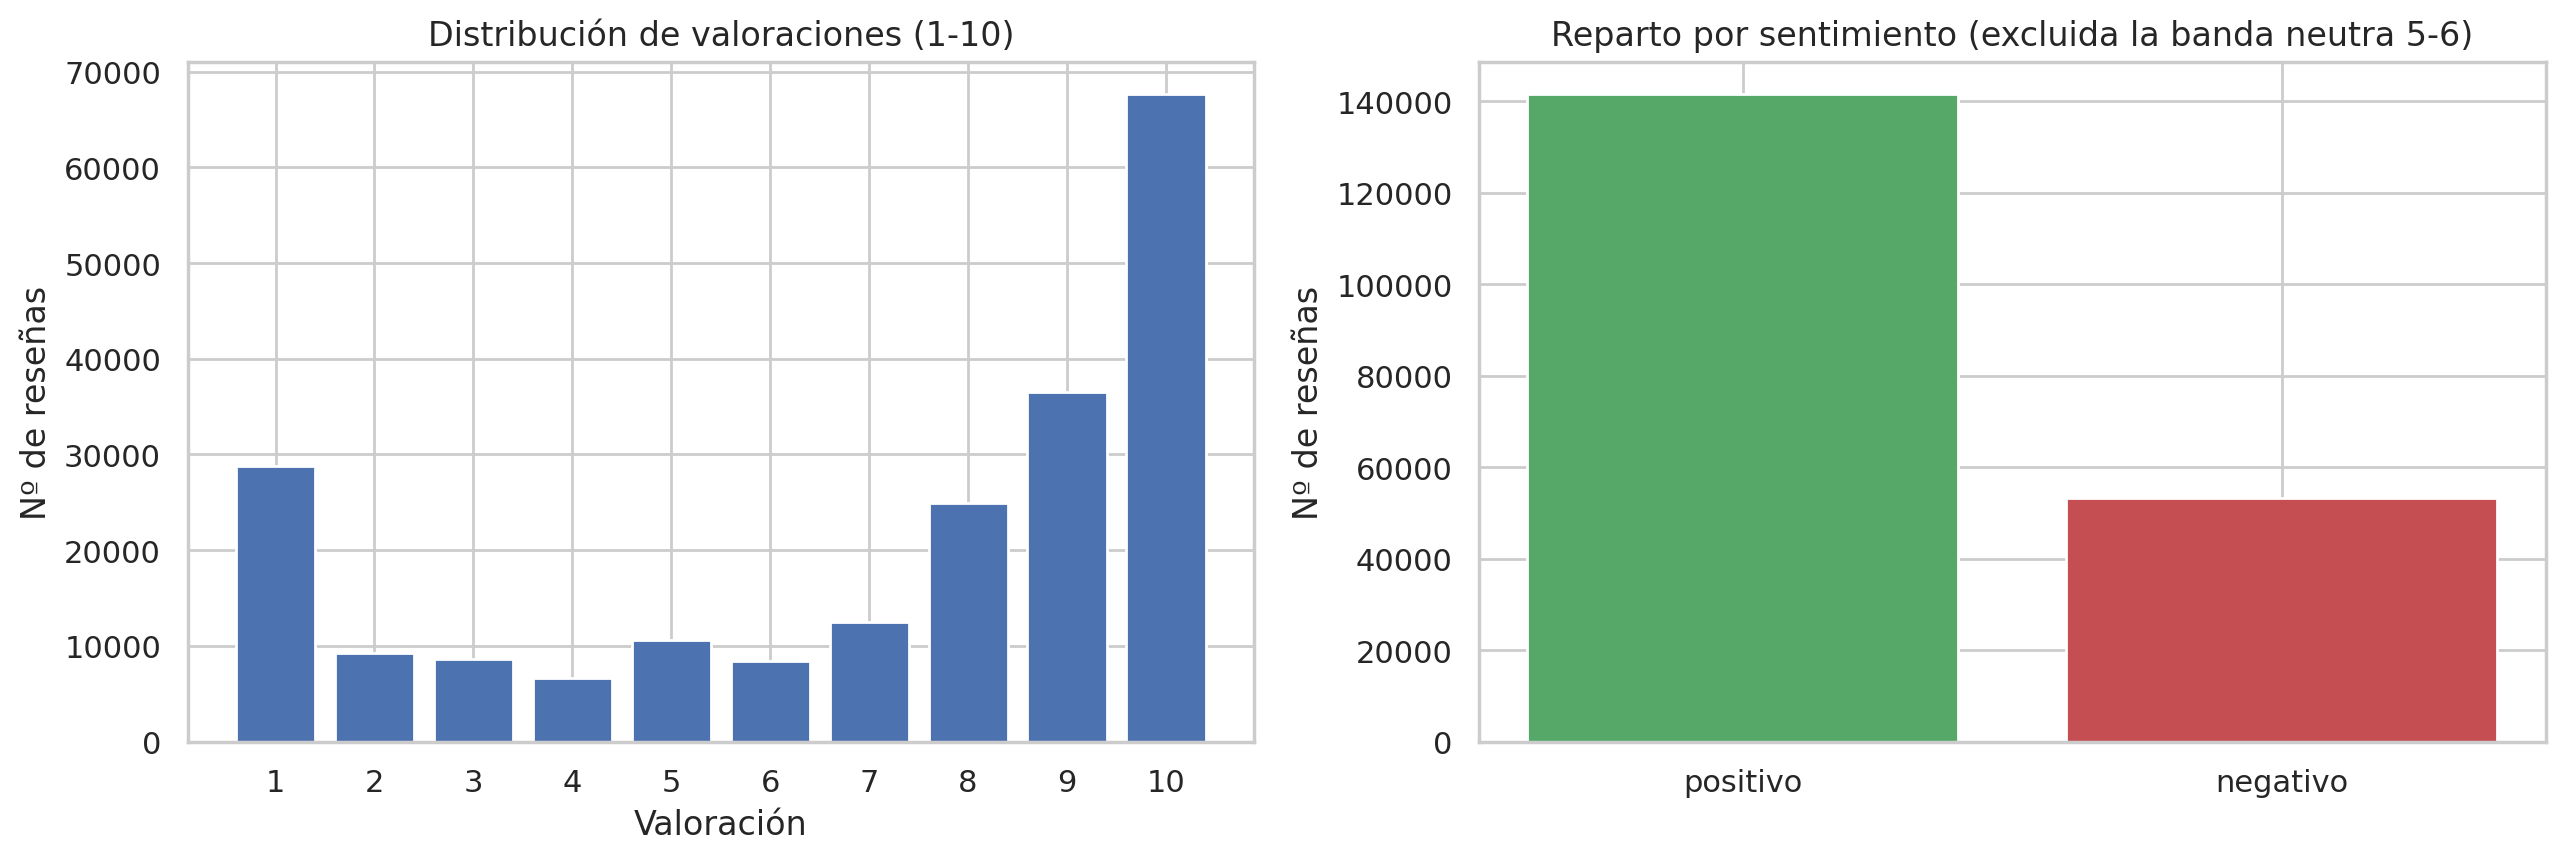
\includegraphics[width=\textwidth]{01_distribucion_ratings}
  \caption{Distribución de valoraciones y reparto por sentimiento.}
  \label{fig:ratings}
\end{figure}

El hallazgo más relevante del análisis exploratorio es que
\textbf{la distribución de valoraciones es marcadamente bimodal}: las
puntuaciones de 10 y de 1 concentran los dos mayores volúmenes, mientras que la
zona intermedia está poco poblada. La valoración media es de \textbf{6,99} y la
mediana de \textbf{8}, con una desviación típica de 3,28.

Esto no es un defecto del conjunto de datos: es información. Los pacientes
escriben cuando tienen algo que celebrar o algo que denunciar. Tiene dos
consecuencias directas para el proyecto: justifica plantear el problema como
clasificación binaria (sección~\ref{sec:etiqueta}) y advierte de que el modelo
verá pocos ejemplos de opiniones tibias.

\subsection{Contrastes estadísticos}

Dos hipótesis intuitivas se han contrastado formalmente en lugar de darlas por
buenas a partir de un gráfico.

\textbf{¿Son más largas las reseñas negativas?} La intuición dice que el
descontento se explaya más. Los datos dicen lo contrario: la mediana es de
\textbf{86 palabras en las positivas} frente a \textbf{79 en las negativas}. La
prueba de Mann-Whitney rechaza la igualdad de distribuciones con
$p = 8{,}03 \times 10^{-90}$. La diferencia es pequeña en magnitud pero
estadísticamente indiscutible: con 194.759 observaciones, casi cualquier
diferencia resulta significativa, motivo por el que se reporta también el
tamaño del efecto y no solo el $p$-valor.

\textbf{¿Se perciben como más útiles las opiniones extremas?} Sí. La
correlación de Spearman entre valoración y número de votos de utilidad es
$\rho = 0{,}28$, y las reseñas extremas (1, 2, 9 o 10) acumulan una media de
\textbf{30,8 votos útiles} frente a \textbf{22,7} de las moderadas.

\subsection{Satisfacción por condición médica}

\begin{figure}[htbp]\centering
  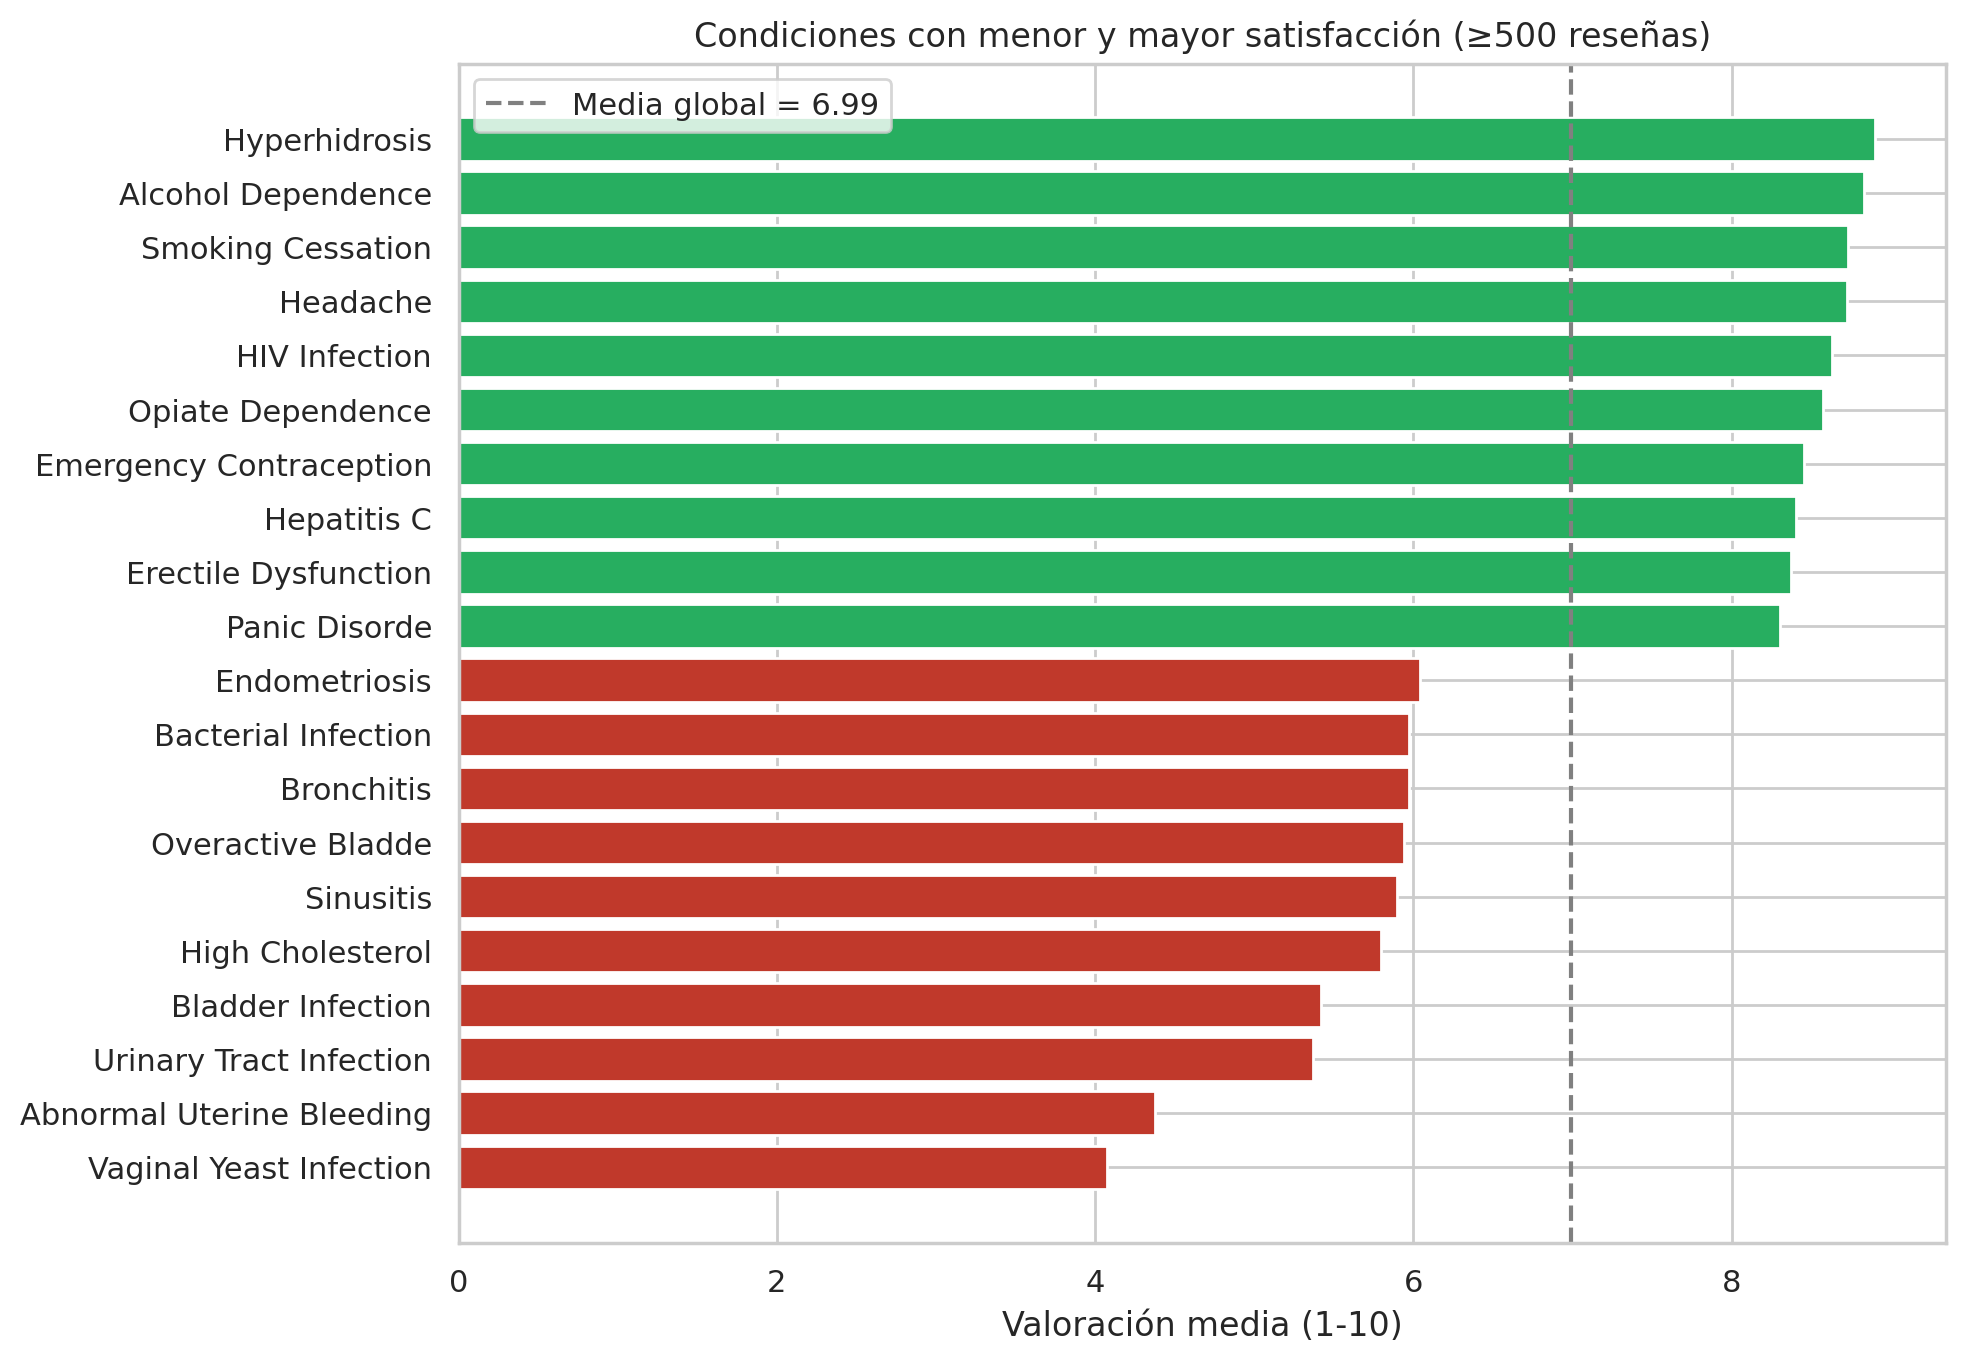
\includegraphics[width=0.92\textwidth]{03_satisfaccion_por_condicion}
  \caption{Condiciones con menor y mayor satisfacción declarada
           (mínimo 500 reseñas).}
\end{figure}

Las diferencias son grandes y clínicamente coherentes. En el extremo inferior
aparecen \textit{Vaginal Yeast Infection} (media 4,08 sobre 3.085 reseñas) y
\textit{Abnormal Uterine Bleeding} (4,38). En el superior, \textit{Hyperhidrosis}
(8,90), \textit{Alcohol Dependence} (8,83) y \textit{Smoking Cessation} (8,73).

El patrón sugiere que la satisfacción es alta cuando el tratamiento resuelve un
problema concreto y verificable por el propio paciente, y baja en condiciones
recurrentes donde el alivio es temporal.

% =====================================================================
\section{Metodología}
% =====================================================================

\subsection{De la valoración a la etiqueta de sentimiento}\label{sec:etiqueta}

Se traduce la valoración numérica en una etiqueta binaria: \textbf{positiva} si
$\text{rating} \geq 7$ y \textbf{negativa} si $\text{rating} \leq 4$. La banda
intermedia (5--6) se descarta por ambigua.

Esta decisión tiene un coste que conviene explicitar: se apartan
\textbf{19.048 reseñas} (el 8,9\% del total). A cambio, las dos clases
representan opiniones inequívocas y la etiqueta resultante es fiable. El
conjunto etiquetado queda en \textbf{194.759 reseñas}, con un
\textbf{72,7\% de positivas}: un desbalanceo moderado que obliga a no evaluar
por \textit{accuracy} y a usar \texttt{class\_weight="balanced"}.

\subsection{Partición: por qué una división aleatoria engaña}\label{sec:particion}

Una partición aleatoria permitiría que el mismo medicamento apareciese en
entrenamiento y en test. El modelo aprendería el vocabulario característico de
ese fármaco —los efectos concretos que produce, cómo lo nombran los pacientes—
y obtendría en test una nota que no reflejaría su capacidad real.

Se ha empleado por ello una \textbf{partición agrupada por medicamento}
(\texttt{GroupShuffleSplit}, 80/20). El resultado: 158.432 reseñas de
entrenamiento y 36.327 de test, con \textbf{721 medicamentos que aparecen
únicamente en test}.

\ideaclave{Evaluar sobre medicamentos nunca vistos produce cifras más bajas que
una partición aleatoria, pero son las únicas que anticipan el comportamiento
real del sistema cuando llegue al mercado un fármaco nuevo.}

\subsection{Representación del texto}

Se emplea \textbf{TF-IDF} con unigramas y bigramas, produciendo una matriz de
$158.432 \times 192.396$. Las decisiones relevantes:

\begin{itemize}[nosep,leftmargin=*]
  \item \texttt{ngram\_range=(1,2)}: los bigramas capturan negaciones y
        expresiones compuestas (\textit{"stopped taking"}, \textit{"weight gain"})
        que un unigrama pierde. Su peso en el modelo final lo confirma.
  \item \texttt{min\_df=5} y \texttt{max\_df=0.9}: descartan erratas
        irrepetibles y términos omnipresentes sin capacidad discriminante.
  \item \texttt{sublinear\_tf=True}: amortigua el efecto de repetir una palabra
        muchas veces dentro de una misma reseña.
\end{itemize}

El vectorizador se ajusta \textbf{únicamente sobre el conjunto de
entrenamiento} y se reutiliza para todos los modelos. Nunca ve el test, por lo
que no existe fuga de información.

\subsection{Modelos evaluados}

\begin{table}[htbp]\centering\small
\caption{Técnicas evaluadas, con sus bondades y debilidades.}
\begin{tabular}{@{}p{2.9cm}p{5.3cm}p{5.3cm}@{}}
\toprule
\textbf{Técnica} & \textbf{Bondades} & \textbf{Debilidades} \\ \midrule
Baseline & Referencia mínima imprescindible & Sin capacidad predictiva \\
Naive Bayes (Complement) & Muy rápido; corrige el sesgo del NB ante clases desbalanceadas & Asume independencia entre términos, falsa en lenguaje natural \\
Regresión Logística & Interpretable; sus coeficientes explican la decisión & Solo capta relaciones lineales \\
SVM lineal & Muy eficaz en alta dimensión & No da probabilidades sin calibrar; calibrar triplica el coste \\
Random Forest (sobre LSA) & Capta interacciones no lineales & Exige reducir dimensionalidad; pierde interpretabilidad \\ \bottomrule
\end{tabular}
\end{table}

Random Forest merece una nota. Aplicarlo directamente sobre 192.396 columnas
dispersas resulta inviable en tiempo y rinde mal. Se le antepone una reducción
de dimensionalidad mediante \texttt{TruncatedSVD} a 150 componentes —Análisis
Semántico Latente—, que es la práctica habitual para combinar modelos de
árboles con representaciones de texto. Se limita además la profundidad de los
árboles a 14 niveles: sin ese límite el entrenamiento supera los cinco minutos
sin mejora apreciable.

Conviene anticipar aquí un dato que resultará decisivo en los resultados: esas
150 componentes explican únicamente el \textbf{8,4\% de la varianza} original.
La compresión es agresiva y, como se verá, tiene un coste.

% =====================================================================
\section{Resultados}
% =====================================================================

\begin{table}[htbp]\centering\small
\caption{Métricas sobre el conjunto de test (36.327 reseñas,
         721 medicamentos no vistos).}
\begin{tabular}{@{}lcccccc@{}}
\toprule
\textbf{Modelo} & \textbf{Accuracy} & \textbf{Precisión} & \textbf{Recall} & \textbf{F1} & \textbf{F1 macro} & \textbf{ROC-AUC} \\ \midrule
Baseline (clase mayoritaria) & 0,7610 & 0,7610 & 1,0000 & 0,8643 & 0,4321 & 0,5000 \\
Random Forest (sobre LSA)    & 0,8578 & 0,9227 & 0,8876 & 0,9048 & 0,8122 & 0,9092 \\
Naive Bayes (Complement)     & 0,8594 & 0,9358 & 0,8753 & 0,9045 & 0,8189 & 0,9235 \\
Regresión Logística          & 0,9171 & 0,9608 & 0,9291 & 0,9446 & \textbf{0,8900} & 0,9647 \\
\textbf{SVM lineal}          & \textbf{0,9221} & 0,9379 & \textbf{0,9613} & \textbf{0,9494} & 0,8898 & \textbf{0,9649} \\ \bottomrule
\end{tabular}
\end{table}

\begin{figure}[htbp]\centering
  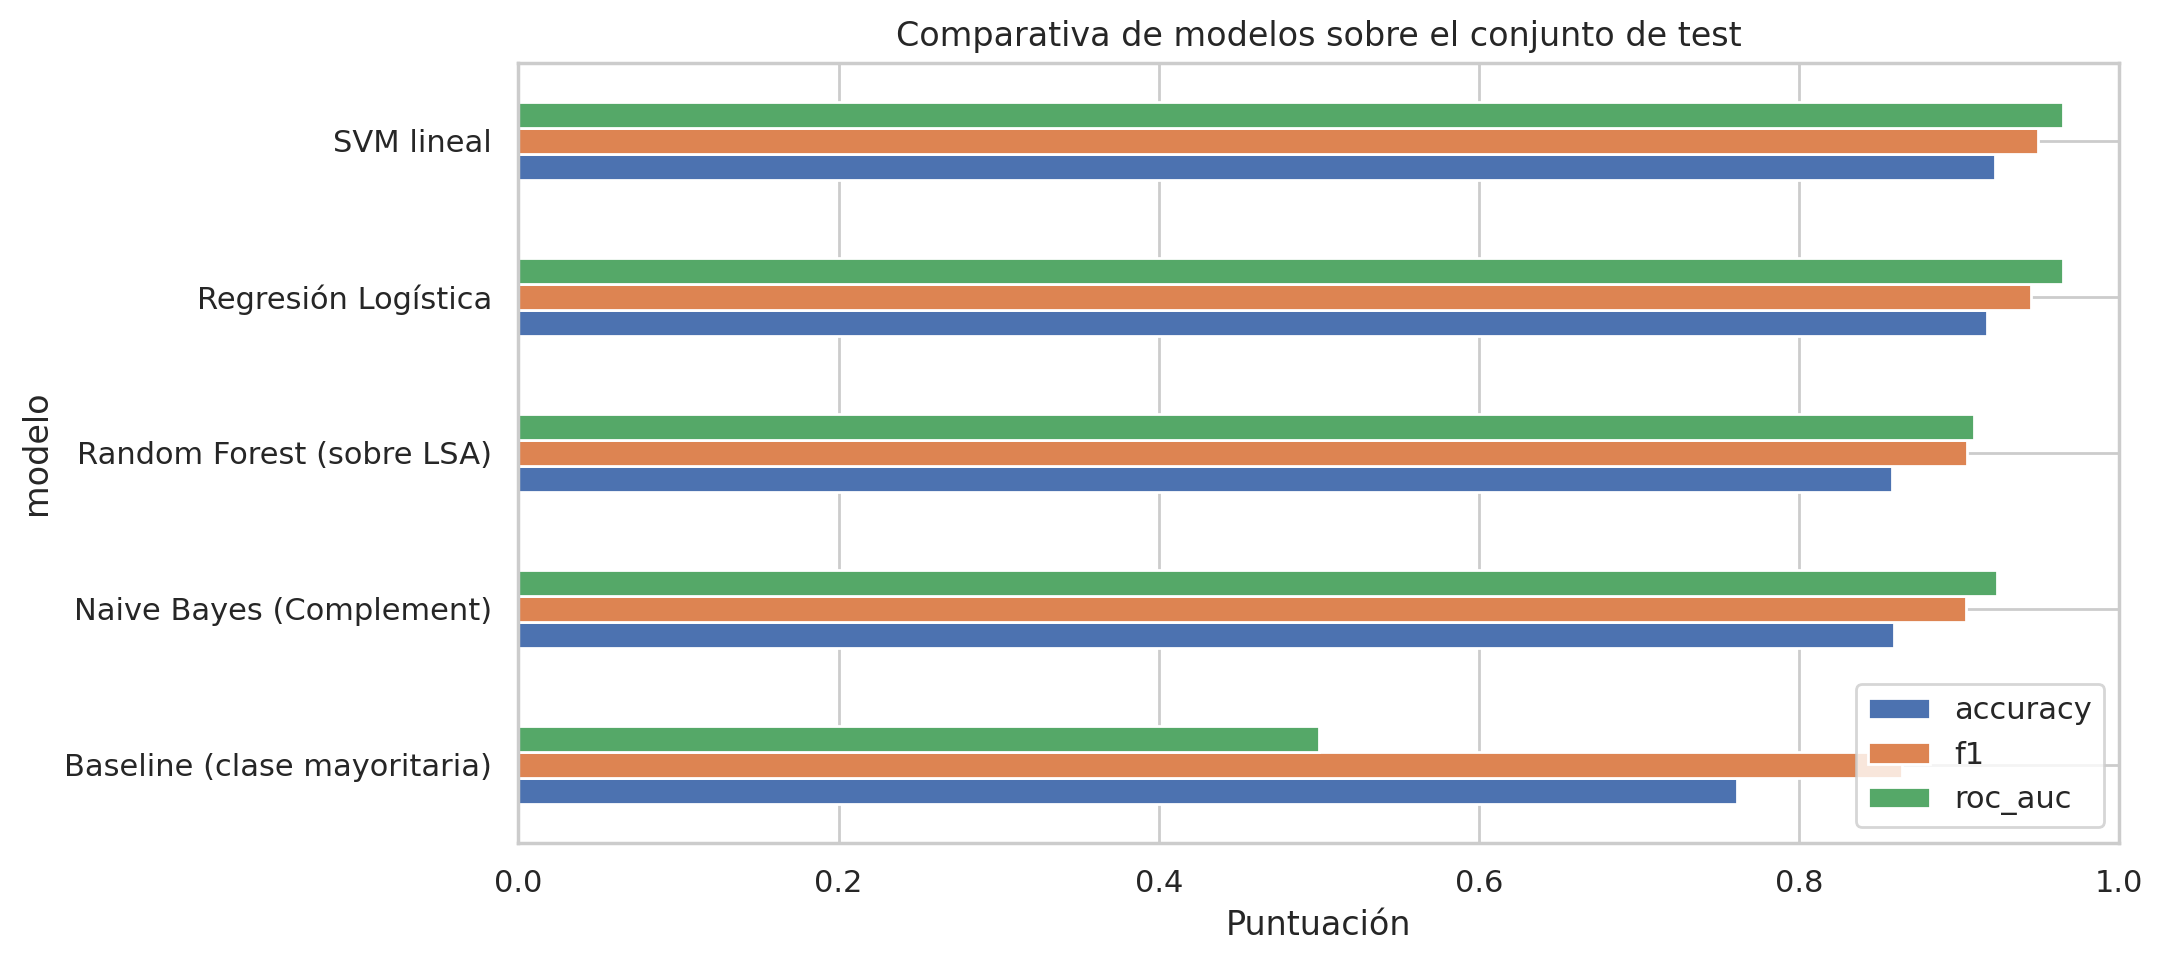
\includegraphics[width=0.95\textwidth]{06_comparativa_modelos}
  \caption{Comparativa de modelos sobre el conjunto de test.}
\end{figure}

\textbf{El baseline ilustra por qué no basta con la \textit{accuracy}.} Predecir
siempre "positivo" alcanza un F1 de 0,8643, una cifra aparentemente buena que
corresponde a un modelo sin ningún valor: su ROC-AUC es 0,5, el del azar. Toda
comparación honesta debe apoyarse en ROC-AUC y F1-macro.

La \textbf{SVM lineal} obtiene el mejor F1 (0,9494) y ROC-AUC (0,9649). La
Regresión Logística queda muy cerca (0,9446 y 0,9647) con una diferencia
prácticamente irrelevante en la práctica, lo que resulta útil: si se
priorizase la interpretabilidad directa, cambiar a Regresión Logística costaría
menos de medio punto de F1.

La validación cruzada de 5 particiones sobre el entrenamiento confirma la
estabilidad: $F1 = 0{,}9358 \pm 0{,}0006$.

\subsection{El modelo no lineal no aporta: por qué}

\textbf{Random Forest queda claramente por detrás} (F1 de 0,9048 y ROC-AUC de
0,9092), al nivel del Naive Bayes y a más de cuatro puntos de ROC-AUC de los
modelos lineales. El resultado merece explicación, porque contradice la
intuición de que un modelo más flexible debería rendir mejor.

La causa no es el algoritmo, sino la representación que se ve obligado a usar.
Random Forest no puede operar sobre 192.396 columnas dispersas, de modo que
antes hay que comprimir el texto a 150 componentes mediante SVD, y esa
compresión \textbf{retiene apenas el 8,4\% de la varianza}. El modelo trabaja,
por tanto, con una versión muy empobrecida de la información: pierde
exactamente los términos poco frecuentes pero muy discriminantes
(\textit{miracle}, \textit{useless}, \textit{ruined}) sobre los que se apoyan
los modelos lineales.

\ideaclave{En clasificación de texto, la capacidad de un modelo para captar
relaciones no lineales importa menos que su capacidad para trabajar
directamente sobre una representación dispersa de alta dimensión. La
flexibilidad del algoritmo no compensa la información destruida al comprimir.}

Su peor comportamiento se concentra además en la clase minoritaria: la
precisión sobre reseñas negativas cae a 0,6807, frente al 0,8661 de la SVM.
Dicho de otro modo, una de cada tres alertas que generaría sería falsa.

\subsection{Dónde se equivoca el modelo}

Las métricas agregadas esconden un desequilibrio importante entre clases:

\begin{table}[htbp]\centering\small
\caption{Rendimiento por clase del modelo seleccionado (SVM lineal).}
\begin{tabular}{@{}lcccc@{}}
\toprule
\textbf{Clase} & \textbf{Precisión} & \textbf{Recall} & \textbf{F1} & \textbf{Casos} \\ \midrule
Negativa & 0,8661 & 0,7972 & 0,8302 & 8.683 \\
Positiva & 0,9379 & 0,9613 & 0,9494 & 27.644 \\ \bottomrule
\end{tabular}
\end{table}

\textbf{El modelo es notablemente peor detectando reseñas negativas}: recupera
el 79,7\% de ellas frente al 96,1\% de las positivas. Dicho de otro modo,
\textbf{una de cada cinco opiniones desfavorables pasa desapercibida}. El F1
macro (0,8898) refleja esta realidad mucho mejor que el F1 global.

Esto importa, y mucho, para el caso de uso: en farmacovigilancia el error caro
es precisamente el falso negativo, la señal de alarma que no se detecta. La
sección~\ref{sec:productivizacion} explica cómo la aplicación mitiga este
problema mediante un umbral de alerta configurable en lugar del 0,5 por defecto.

% =====================================================================
\section{Interpretabilidad: por qué decide lo que decide}
% =====================================================================

\begin{figure}[htbp]\centering
  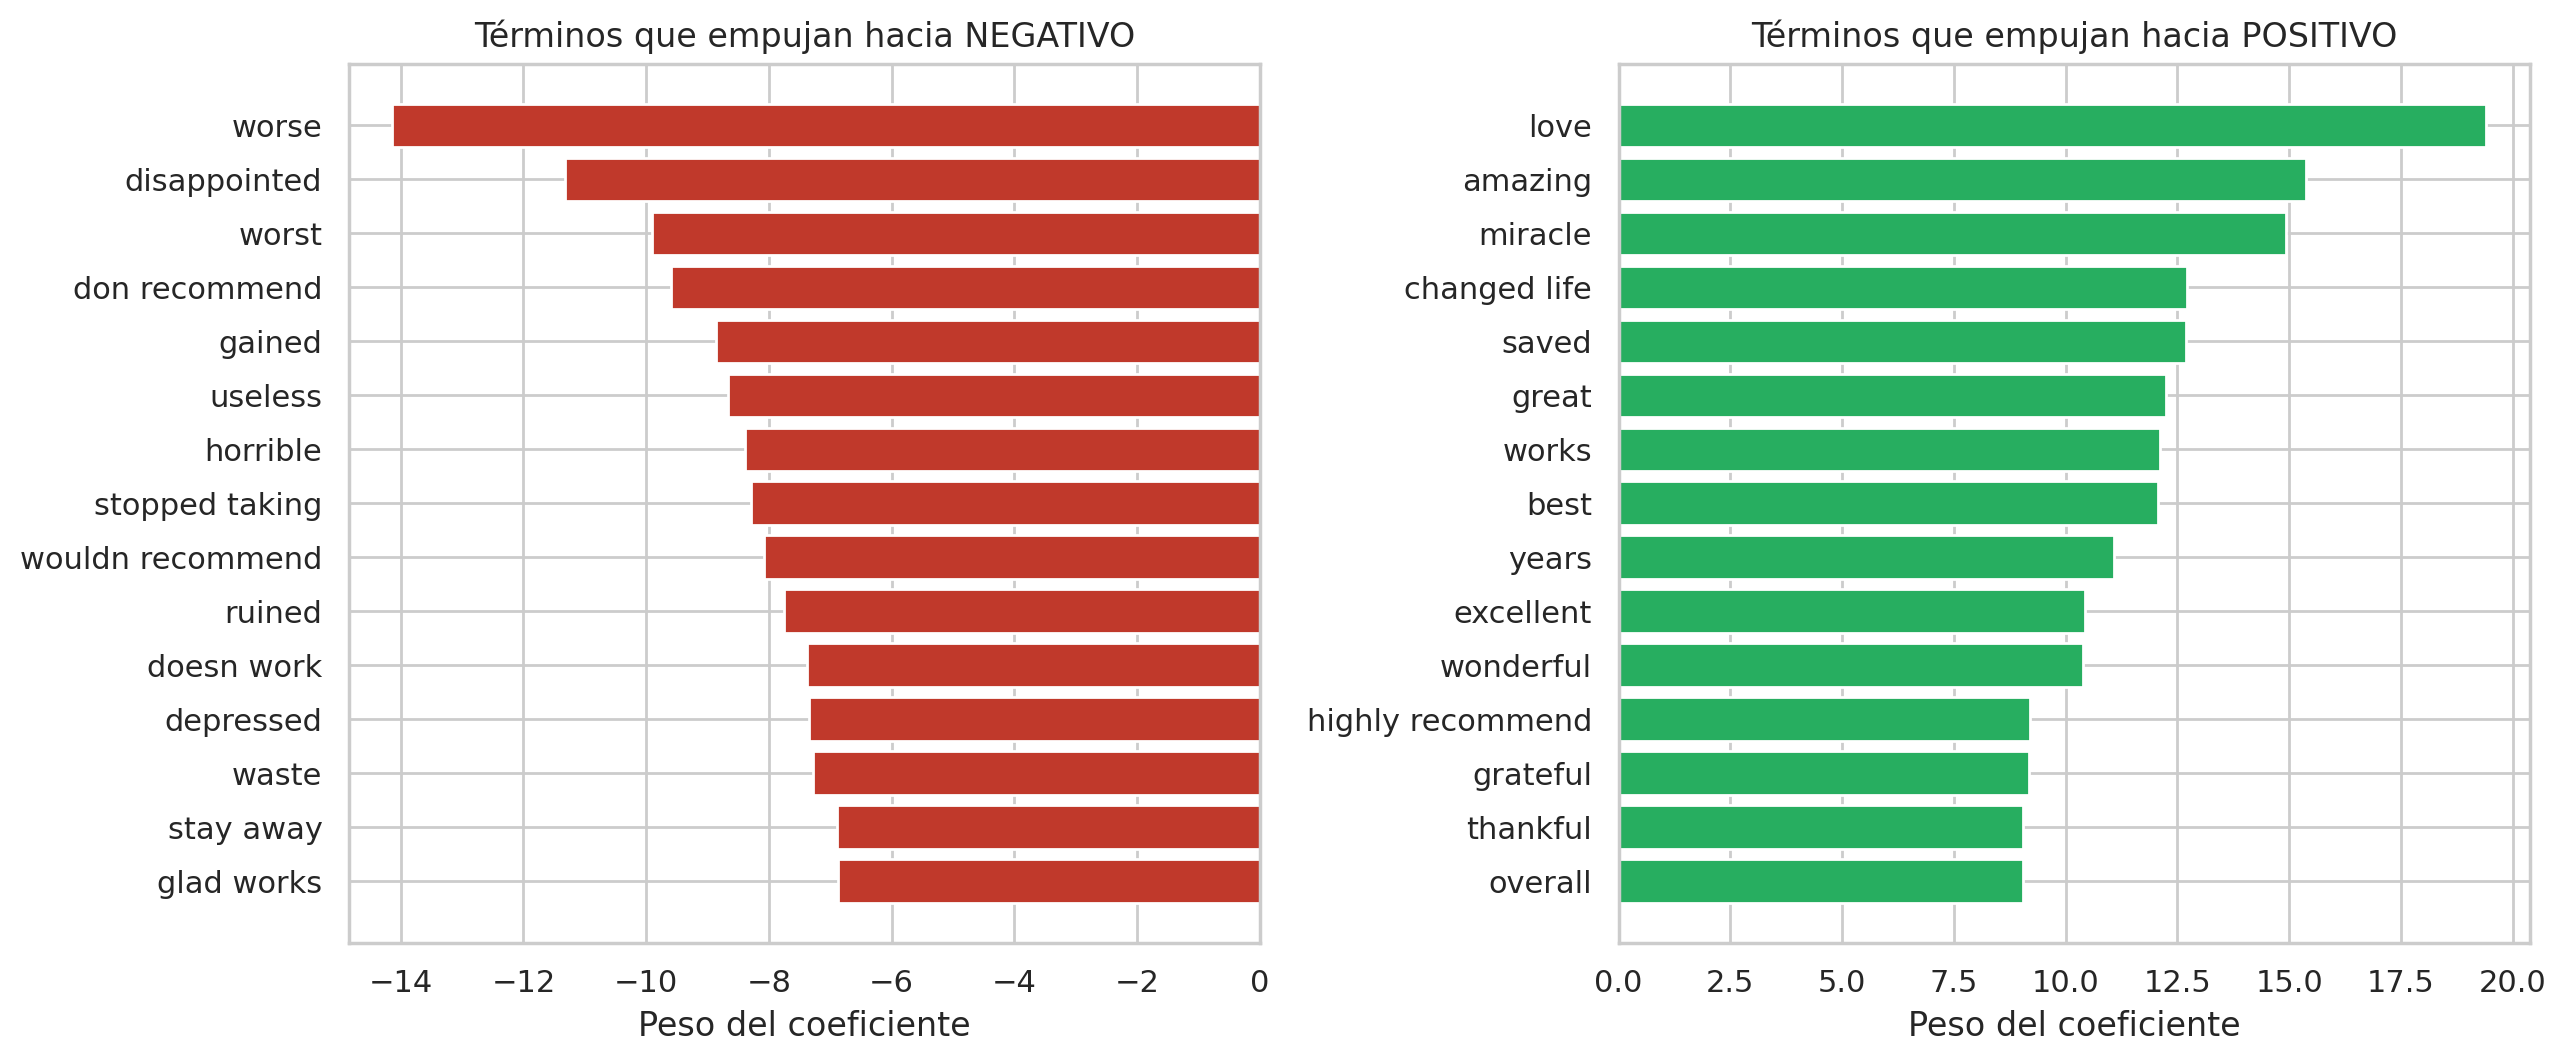
\includegraphics[width=\textwidth]{09_terminos_influyentes}
  \caption{Términos con mayor peso en la decisión del modelo.}
\end{figure}

Como la SVM calibrada no expone coeficientes directamente interpretables, la
explicabilidad global se calcula sobre la Regresión Logística, cuyo rendimiento
es equivalente. Los términos aprendidos son un buen indicio de que el modelo
capta señal real y no artefactos:

\begin{itemize}[nosep,leftmargin=*]
  \item \textbf{Hacia negativo:} \textit{worse}, \textit{disappointed},
        \textit{worst}, \textit{don't recommend}, \textit{gained},
        \textit{useless}, \textit{horrible}, \textit{stopped taking},
        \textit{ruined}.
  \item \textbf{Hacia positivo:} \textit{love}, \textit{amazing},
        \textit{miracle}, \textit{changed life}, \textit{saved},
        \textit{great}, \textit{works}, \textit{best}, \textit{excellent}.
\end{itemize}

Obsérvese que varios de los términos más informativos son \textbf{bigramas}
(\textit{"stopped taking"}, \textit{"changed life"}, \textit{"don't recommend"}),
lo que valida la decisión de incluirlos en la representación.

\subsection{Explicación de un caso concreto}

Sobre una reseña real de \textbf{Apixaban} con valoración 1, el modelo asigna
una probabilidad de sentimiento positivo de \textbf{0,079}, es decir, la
clasifica correctamente como negativa con alta confianza. Los términos que más
pesan en esa decisión son \textit{stop}, \textit{developed}, \textit{taking} y
\textit{flu}, coherentes con un relato de abandono del tratamiento por efectos
adversos.

Este nivel de explicación es lo que permite que un revisor humano confíe en el
sistema: no recibe un veredicto opaco, sino un veredicto con sus motivos.

% =====================================================================
\section{Temas y aspectos en las opiniones}\label{sec:aspectos}
% =====================================================================

La factorización matricial no negativa (NMF) sobre TF-IDF identifica ocho temas
sin ninguna supervisión. Su nitidez es notable: emergen áreas terapéuticas
reconocibles sin haberlas definido.

\begin{figure}[htbp]\centering
  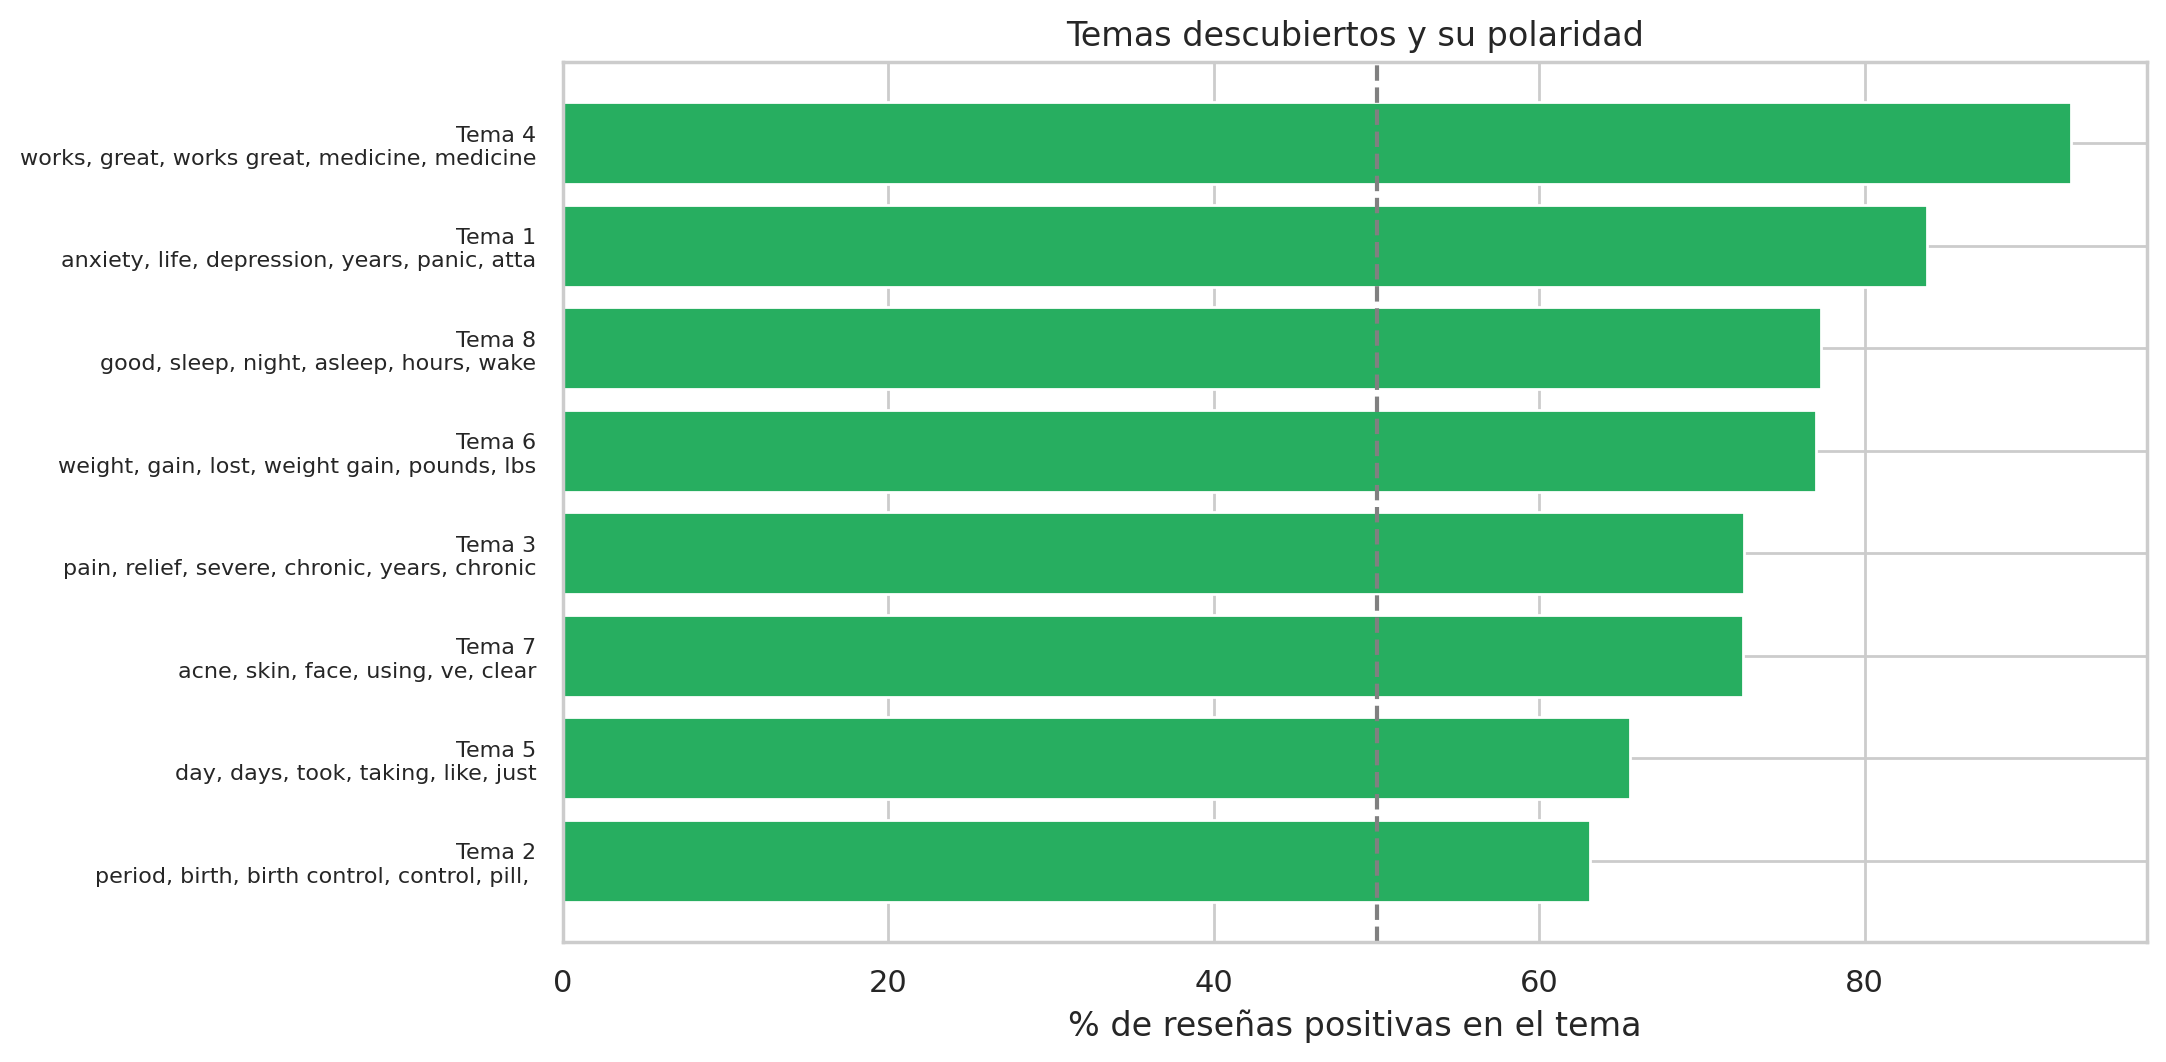
\includegraphics[width=0.95\textwidth]{10_temas_nmf}
  \caption{Temas descubiertos mediante NMF y su polaridad.}
\end{figure}

\begin{table}[htbp]\centering\small
\caption{Temas descubiertos y proporción de reseñas positivas.}
\begin{tabular}{@{}llc@{}}
\toprule
\textbf{Tema} & \textbf{Términos principales} & \textbf{\% positivas} \\ \midrule
Eficacia general      & works, great, medicine works        & 92,7\% \\
Ansiedad y depresión  & anxiety, life, depression, panic    & 83,8\% \\
Sueño                 & sleep, night, asleep, hours         & 77,3\% \\
Peso                  & weight, gain, lost, pounds          & 77,0\% \\
Dolor crónico         & pain, relief, severe, chronic       & 72,6\% \\
Dermatología          & acne, skin, face, clear             & 72,5\% \\
Posología             & day, days, took, taking             & 65,6\% \\
Anticoncepción        & period, birth control, pill         & 63,1\% \\ \bottomrule
\end{tabular}
\end{table}

\subsection{Un hallazgo contraintuitivo}

El análisis por aspectos, construido sobre un léxico definido explícitamente
(véase Anexo~B), arroja el resultado más interesante del trabajo.

\begin{table}[htbp]\centering\small
\caption{Aspectos mencionados y su relación con la valoración.}
\begin{tabular}{@{}lccc@{}}
\toprule
\textbf{Aspecto} & \textbf{\% reseñas} & \textbf{Valoración si lo menciona} & \textbf{Si no} \\ \midrule
Eficacia                   & 51,3\% & 7,58 & 6,69 \\
Efectos secundarios        & 63,5\% & 7,16 & 7,12 \\
Posología y administración & 43,5\% & 7,18 & 7,11 \\
Coste y acceso             &  7,6\% & 7,37 & 7,12 \\ \bottomrule
\end{tabular}
\end{table}

Cabría esperar que mencionar efectos secundarios fuese señal de insatisfacción.
\textbf{No lo es}: la valoración media apenas varía (7,16 frente a 7,12) pese a
que el aspecto aparece en el 63,5\% de las reseñas. Lo que sí discrimina es
hablar de \textbf{eficacia}, con una diferencia de casi un punto (7,58 frente a
6,69).

\ideaclave{Los pacientes toleran los efectos secundarios cuando el medicamento
funciona. Lo que determina la satisfacción no es la ausencia de efectos
adversos, sino la percepción de eficacia. Un sistema de alerta que se limitase
a buscar menciones de efectos secundarios generaría un enorme volumen de falsos
positivos.}

\begin{figure}[htbp]\centering
  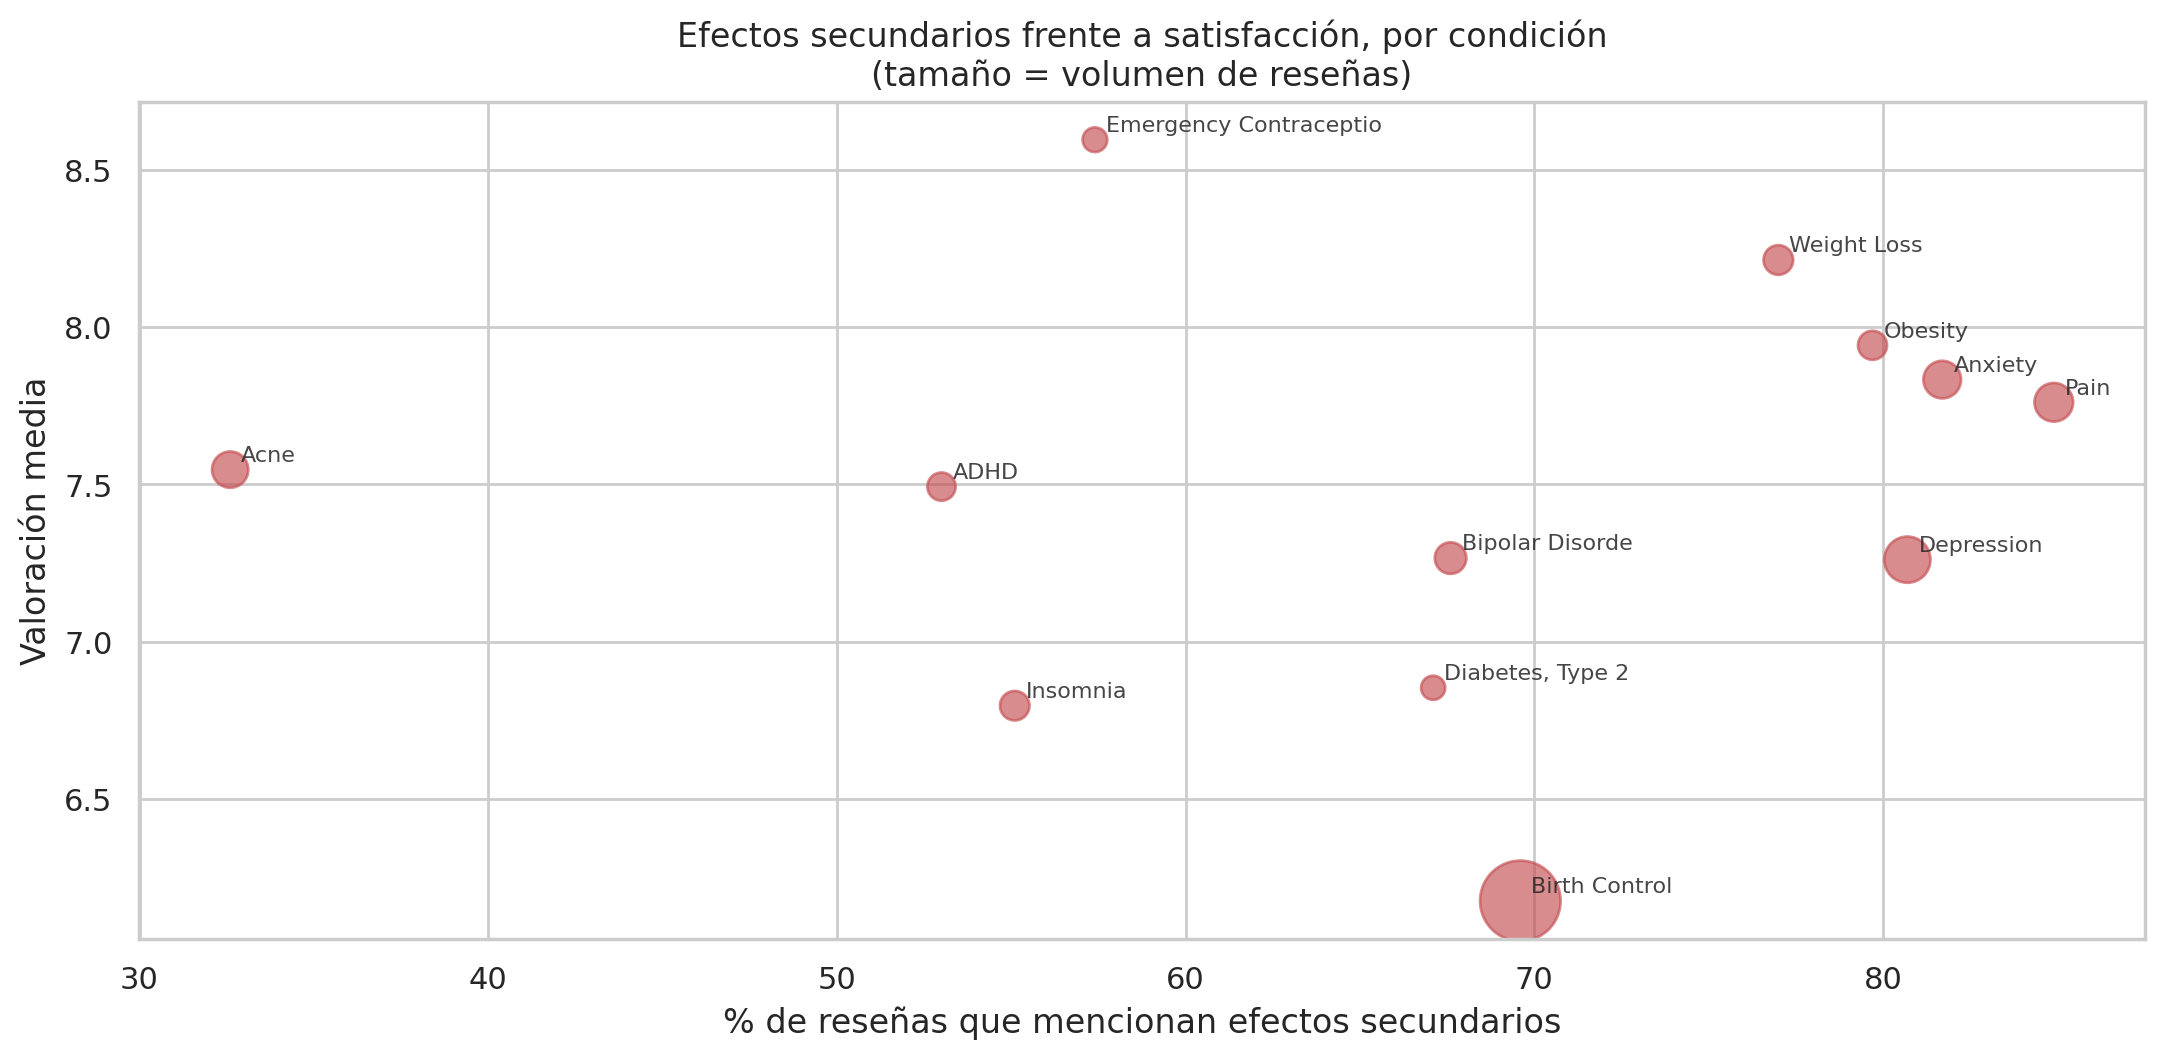
\includegraphics[width=0.95\textwidth]{12_aspectos_por_condicion}
  \caption{Menciones de efectos secundarios frente a satisfacción, por condición.}
\end{figure}

El cruce por condición señala dónde mirar. \textbf{Birth Control} destaca como
el caso más preocupante: con 33.573 reseñas —el mayor volumen del corpus—
registra la valoración media más baja del grupo (6,18), un 69,6\% de menciones
de efectos secundarios y solo un 31,3\% de menciones de eficacia. Es
exactamente el perfil que justificaría una revisión: mucho volumen, baja
satisfacción y escasa percepción de que el tratamiento funcione.

% =====================================================================
\section{Productivización}\label{sec:productivizacion}
% =====================================================================

Un modelo que solo vive en un cuaderno de análisis no aporta valor. El modelo
entrenado se ha empaquetado en una \textbf{aplicación web operativa}.

\subsection{Arquitectura}

La solución se serializa como un \textit{pipeline} único
(\texttt{joblib}, 289~KB) que encapsula el vectorizador y el clasificador. Esto
garantiza que el texto recibido en producción atraviese exactamente las mismas
transformaciones que durante el entrenamiento, eliminando la principal fuente
de errores en el despliegue de modelos de NLP.

Sobre él, una interfaz en \textbf{Streamlit} expone tres funciones:
predicción con probabilidad asociada, detección de aspectos y explicación local
mediante LIME.

\subsection{Del texto a la decisión}

% >>> PENDIENTE: inserta aquí dos capturas de la aplicación en funcionamiento
%     (una reseña favorable y otra desfavorable). Ejecuta:
%         streamlit run src/app.py
%     y guarda las capturas en memoria/img/. Después descomenta el bloque:
%
% \begin{figure}[htbp]\centering
%   \includegraphics[width=\textwidth]{img/app_captura}
%   \caption{Aplicación analizando una reseña nueva.}
% \end{figure}

El recorrido de una reseña nueva es inmediato: el analista la pega, y el
sistema devuelve el sentimiento previsto con su probabilidad, los aspectos
detectados y los términos que han inclinado la decisión.

La aplicación incorpora un \textbf{umbral de alerta configurable}
(0,35 por defecto en lugar del 0,5 habitual). Esta decisión responde
directamente a la debilidad identificada en la sección de errores: al elevar la
sensibilidad hacia la clase negativa se recuperan reseñas desfavorables que un
umbral neutro dejaría escapar, a costa de revisar algunos falsos positivos.
En farmacovigilancia, ese intercambio es claramente favorable.

% =====================================================================
\section{Discusión orientada a negocio}
% =====================================================================

\textbf{Volumen procesable.} Sobre las 36.327 reseñas de test, el sistema
identifica correctamente 6.922 de las 8.683 opiniones negativas. Una revisión
manual equivalente, a un ritmo conservador de dos minutos por reseña,
supondría más de 1.200 horas de trabajo.

\textbf{Dónde poner el foco.} El análisis por aspectos redirige el esfuerzo de
vigilancia: rastrear menciones de efectos secundarios es ineficiente porque
aparecen en el 63,5\% de las reseñas sin correlación con la insatisfacción. La
señal útil está en la percepción de eficacia.

\textbf{El coste del error.} Con la configuración por defecto, una de cada
cinco reseñas negativas pasa desapercibida. El sistema debe entenderse como un
\textbf{filtro de priorización}, no como un sustituto del criterio humano: su
valor está en ordenar por urgencia un volumen inabarcable, no en decidir por sí
solo.

\textbf{Respuesta a las preguntas planteadas.} P1: sí, el texto por sí solo
predice la satisfacción con un ROC-AUC de 0,9649. P2: sí, y esa cifra se
obtiene precisamente sobre medicamentos nunca vistos. P3: los aspectos que
concentran la insatisfacción no son los esperados, como se ha discutido.

% =====================================================================
\section{Conclusiones y líneas futuras}
% =====================================================================

\subsection{Conclusiones}

\begin{enumerate}[leftmargin=*]
  \item Es posible predecir la satisfacción de un paciente a partir
        exclusivamente del texto de su reseña, con un \textbf{F1 de 0,9494} y un
        \textbf{ROC-AUC de 0,9649} sobre medicamentos no vistos.
  \item Los modelos lineales sobre TF-IDF resultan muy competitivos en esta
        tarea. La diferencia entre SVM y Regresión Logística es marginal, lo que
        permite elegir en función de la interpretabilidad deseada.
  \item \textbf{Aumentar la complejidad del modelo no mejora el resultado.}
        Random Forest, pese a captar relaciones no lineales, queda cuatro puntos
        de ROC-AUC por detrás porque se ve obligado a trabajar sobre una
        compresión que conserva el 8,4\% de la varianza. En texto, la
        representación pesa más que la sofisticación del algoritmo.
  \item \textbf{Mencionar efectos secundarios no predice insatisfacción}; sí lo
        hace la percepción de eficacia. Es el hallazgo con mayor implicación
        práctica del trabajo.
  \item El desequilibrio entre clases es la principal limitación: el modelo
        detecta peor lo negativo, que es justamente lo que más importa.
\end{enumerate}

\subsection{Lecciones aprendidas}

La decisión técnica con mayor impacto no fue la elección del algoritmo, sino la
\textbf{estrategia de partición}. Comprobar que una división aleatoria inflaba
las métricas obligó a rehacer la evaluación y produjo cifras más bajas, pero
defendibles.

La segunda lección llegó con Random Forest. Entrenarlo directamente sobre la
matriz dispersa resultó inviable, y la reducción necesaria para hacerlo
ejecutable acabó siendo la causa de su peor rendimiento. Es un buen recordatorio
de que una restricción computacional puede convertirse, sin advertirlo, en una
limitación metodológica.

Por último, medir siempre contra un \textit{baseline} trivial evitó un error de
lectura: un F1 de 0,86 parecía un buen resultado hasta comprobar que se
alcanzaba prediciendo siempre la misma clase.

\subsection{Líneas futuras}

\begin{itemize}[nosep,leftmargin=*]
  \item \textbf{Modelos basados en Transformers.} Un modelo tipo BERT ajustado
        al dominio médico debería capturar mejor la negación y la ironía, las
        dos fuentes de error más frecuentes.
  \item \textbf{Umbral optimizado por coste.} Ajustar el umbral maximizando una
        función de coste explícita en lugar de fijarlo heurísticamente.
  \item \textbf{Detección de emergentes.} Vigilar la aparición de términos
        nuevos asociados a un medicamento como señal temprana de un efecto
        adverso no documentado.
  \item \textbf{Extensión multilingüe}, para aplicar el sistema a corpus en
        español.
\end{itemize}

% =====================================================================
\begin{thebibliography}{9}\small
\bibitem{graesser2018} Gräßer, F., Kallumadi, S., Malberg, H., Zaunseder, S. (2018).
  \textit{Aspect-Based Sentiment Analysis of Drug Reviews Applying Cross-Domain
  and Cross-Data Learning}. International Conference on Digital Health, 121--125.
\bibitem{pedregosa2011} Pedregosa, F. et al. (2011). \textit{Scikit-learn:
  Machine Learning in Python}. Journal of Machine Learning Research, 12, 2825--2830.
\bibitem{ribeiro2016} Ribeiro, M. T., Singh, S., Guestrin, C. (2016).
  \textit{“Why Should I Trust You?”: Explaining the Predictions of Any
  Classifier}. KDD 2016, 1135--1144.
\bibitem{lee2001} Lee, D. D., Seung, H. S. (2001). \textit{Algorithms for
  Non-negative Matrix Factorization}. NIPS 13, 556--562.
\end{thebibliography}

% =====================================================================
\newpage
\appendix
\renewcommand{\thesection}{\appendixname~\Alph{section}}

% A partir de aquí la numeración pasa a ser "Anexo A", "Anexo B"..., mucho más
% ancha que un simple "A". Sin ensanchar la columna del índice, el rótulo se
% solaparía con el título. Solo afecta a las entradas de los anexos.
\addtocontents{toc}{\protect\setlength{\protect\cftsecnumwidth}{5.6em}}

% =====================================================================
\section{Código desarrollado y reproducibilidad}
% =====================================================================

% >>> PENDIENTE: sustituye la línea siguiente por la URL real del repositorio
%     una vez lo hayas creado y hayas dado acceso a los tutores.
%     NO entregues la memoria con este texto sin completar.
El código completo se encuentra en el siguiente repositorio:

\vspace{0.2cm}
\begin{center}\ttfamily [URL DEL REPOSITORIO]\end{center}
\vspace{0.2cm}

\vspace{0.2cm}
\begin{center}\small
\begin{tabular}{@{}ll@{}}
\toprule
\textbf{Fichero} & \textbf{Contenido} \\ \midrule
\texttt{src/config.py}   & Rutas, constantes, carga y limpieza de datos \\
\texttt{src/eda.py}      & Fase 1: análisis descriptivo y contrastes \\
\texttt{src/modelado.py} & Fase 2: vectorización y comparativa de modelos \\
\texttt{src/topics\_explicabilidad.py} & Fase 3: temas, aspectos y LIME \\
\texttt{src/app.py}      & Fase 4: aplicación de productivización \\ \bottomrule
\end{tabular}
\end{center}

\textbf{Reproducción completa} en cuatro órdenes:

\vspace{0.15cm}
{\small\ttfamily
pip install -r requirements.txt\\
python src/eda.py\\
python src/modelado.py\\
python src/topics\_explicabilidad.py
}
\vspace{0.15cm}

Todos los procesos aleatorios emplean la semilla fija
\texttt{RANDOM\_STATE = 42}: partición, submuestreos, NMF, SVD, Random Forest y
LIME. Las métricas se escriben en \texttt{resultados/metricas/*.json}, de modo
que \textbf{cada cifra de esta memoria es trazable hasta una ejecución concreta}
y puede verificarse volviendo a ejecutar el código.

% =====================================================================
\section{Léxico de aspectos}
% =====================================================================

El análisis de la sección~\ref{sec:aspectos} se apoya en un léxico definido de
forma explícita. Se optó por esta vía —y no por un diccionario automático—
porque el objetivo era medir aspectos concretos y accionables para
farmacovigilancia, no obtener categorías genéricas.

La búsqueda se realiza sobre el texto en minúsculas mediante expresiones
regulares con delimitadores de palabra (\texttt{$\backslash$b}), de forma que
\textit{"pain"} no active una coincidencia dentro de \textit{"painting"}.

\vspace{0.25cm}
\begin{center}\small
\begin{tabular}{@{}p{3.3cm}p{10.5cm}@{}}
\toprule
\textbf{Aspecto} & \textbf{Términos} \\ \midrule
Eficacia & work, works, worked, effective, helped, help, relief, improve,
           improved, better, cured, results \\ \addlinespace
Efectos secundarios & side, effects, nausea, headache, dizzy, dizziness, weight,
           gain, anxiety, insomnia, tired, fatigue, pain, sick, vomiting, rash,
           depression \\ \addlinespace
Posología y administración & dose, dosage, mg, pill, pills, tablet, injection,
           daily, twice, morning, night, taper, withdrawal \\ \addlinespace
Coste y acceso & price, cost, expensive, insurance, cheap, afford, pharmacy,
           generic, coupon \\ \bottomrule
\end{tabular}
\end{center}

\vspace{0.3cm}
\textbf{Limitación conocida.} El léxico detecta la \textit{mención} de un
aspecto, no su \textit{polaridad}: la frase \textit{"no side effects"} cuenta
como mención de efectos secundarios. Esta es, muy probablemente, una de las
razones por las que dicho aspecto apenas discrimina entre reseñas satisfechas e
insatisfechas (Tabla~6). Un análisis de sentimiento basado en aspectos, con
detección de negación, es la extensión natural de este trabajo.

% =====================================================================
\section{Análisis exploratorio ampliado}
% =====================================================================

\begin{figure}[htbp]\centering
  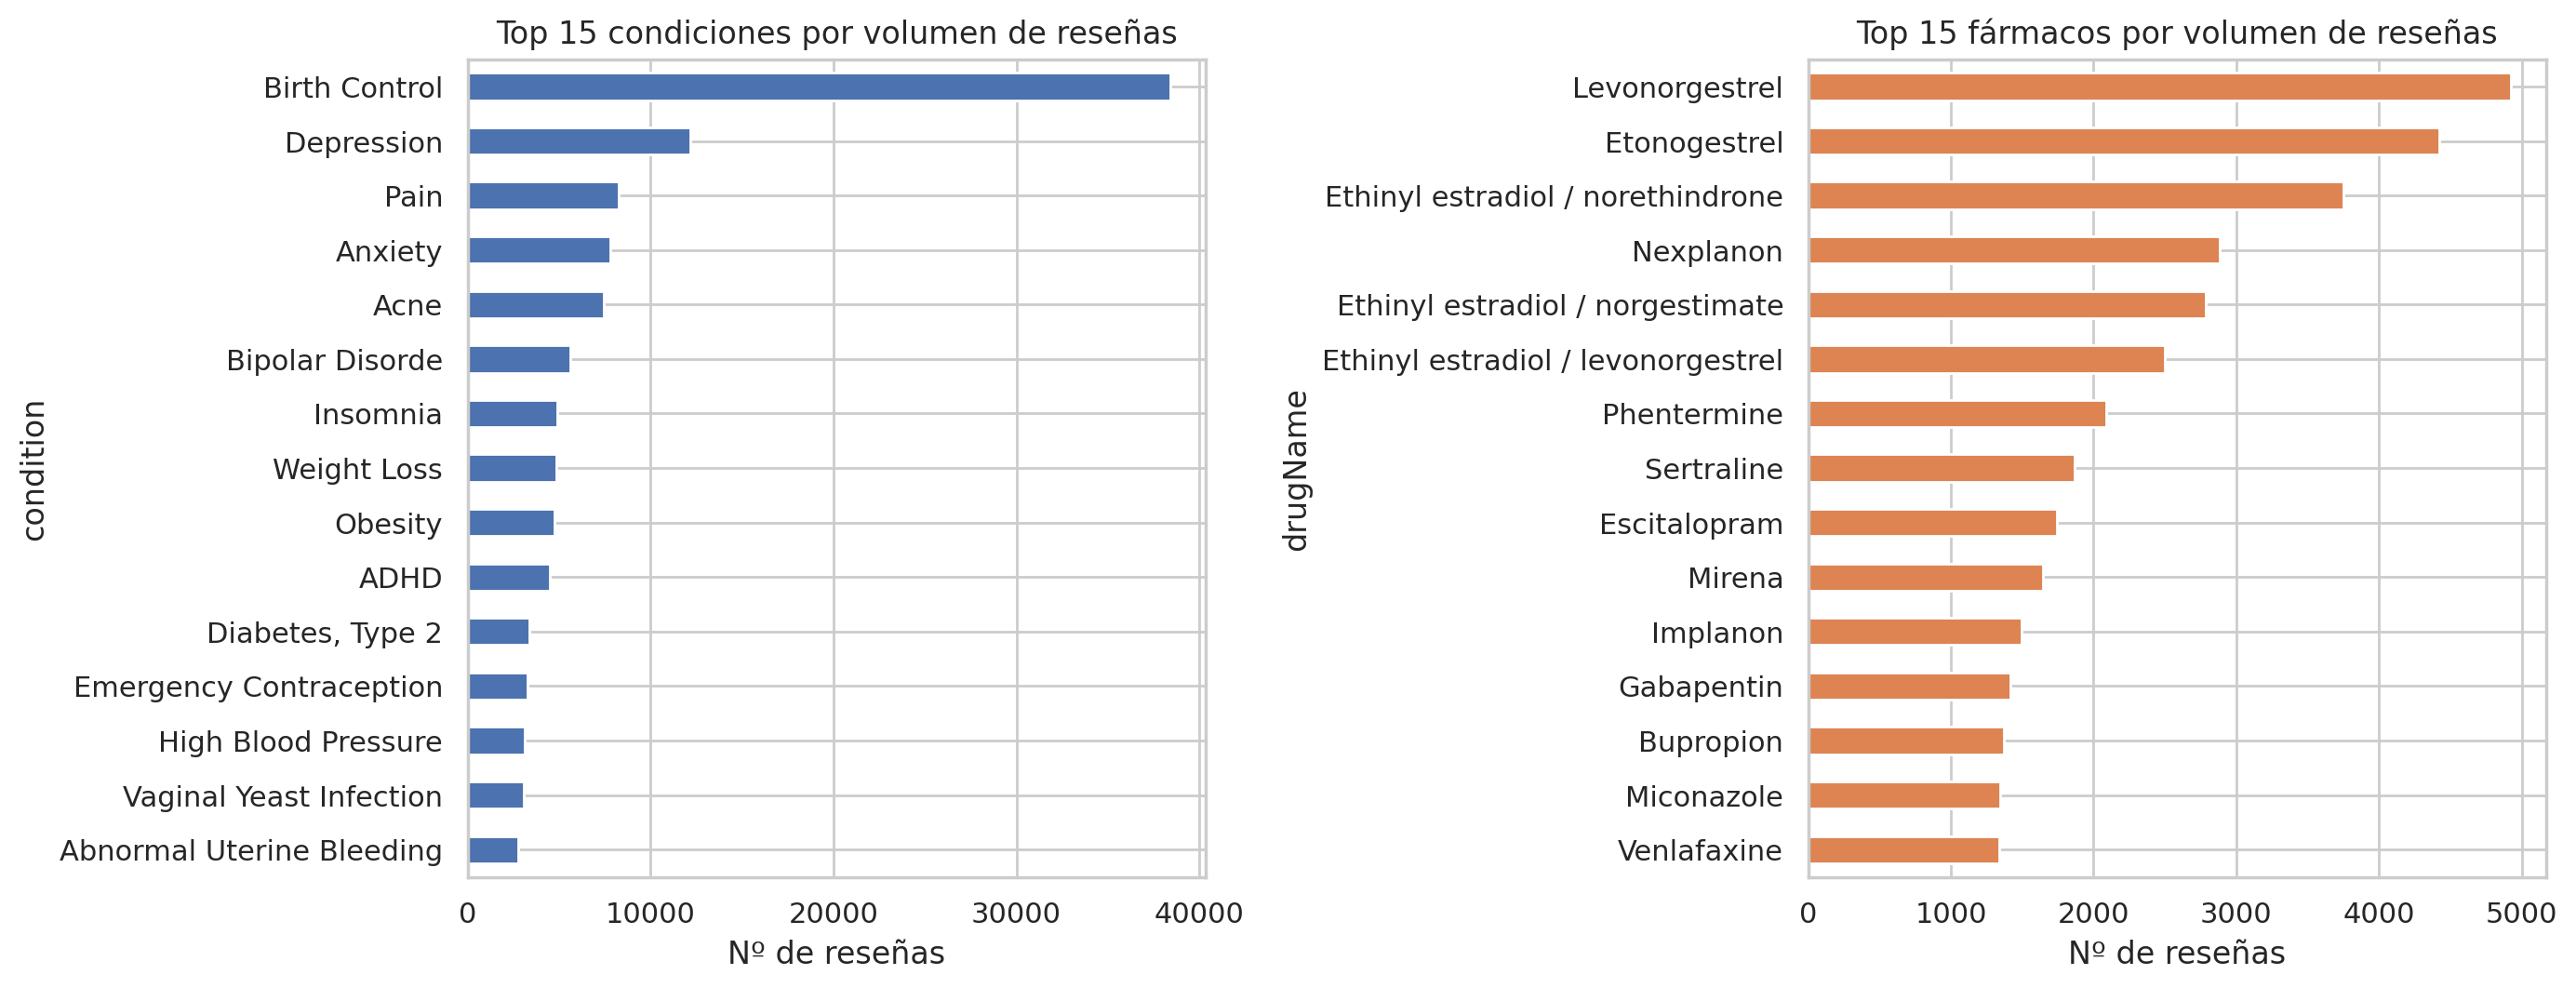
\includegraphics[width=\textwidth]{02_top_condiciones_farmacos}
  \caption{Condiciones y medicamentos con mayor volumen de reseñas.}
\end{figure}

\begin{figure}[htbp]\centering
  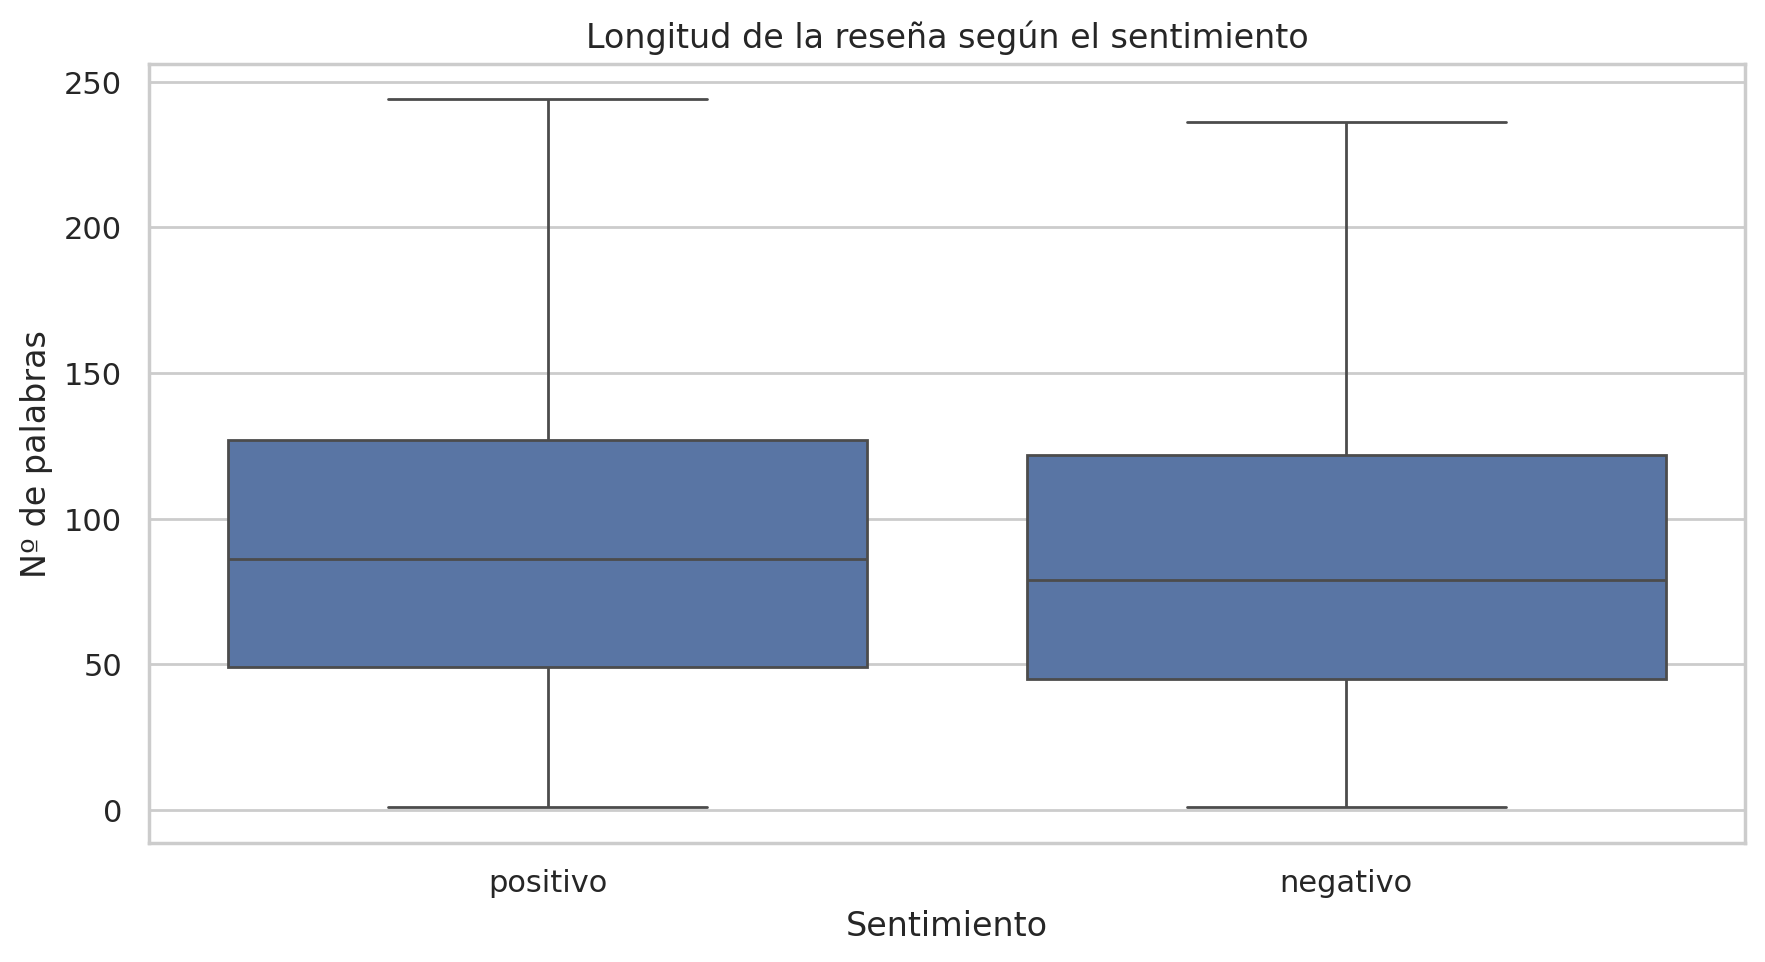
\includegraphics[width=0.75\textwidth]{04_longitud_vs_sentimiento}
  \caption{Distribución de la longitud de la reseña según el sentimiento.
           Base gráfica del contraste de Mann-Whitney de la sección~4.1.}
\end{figure}

\begin{figure}[htbp]\centering
  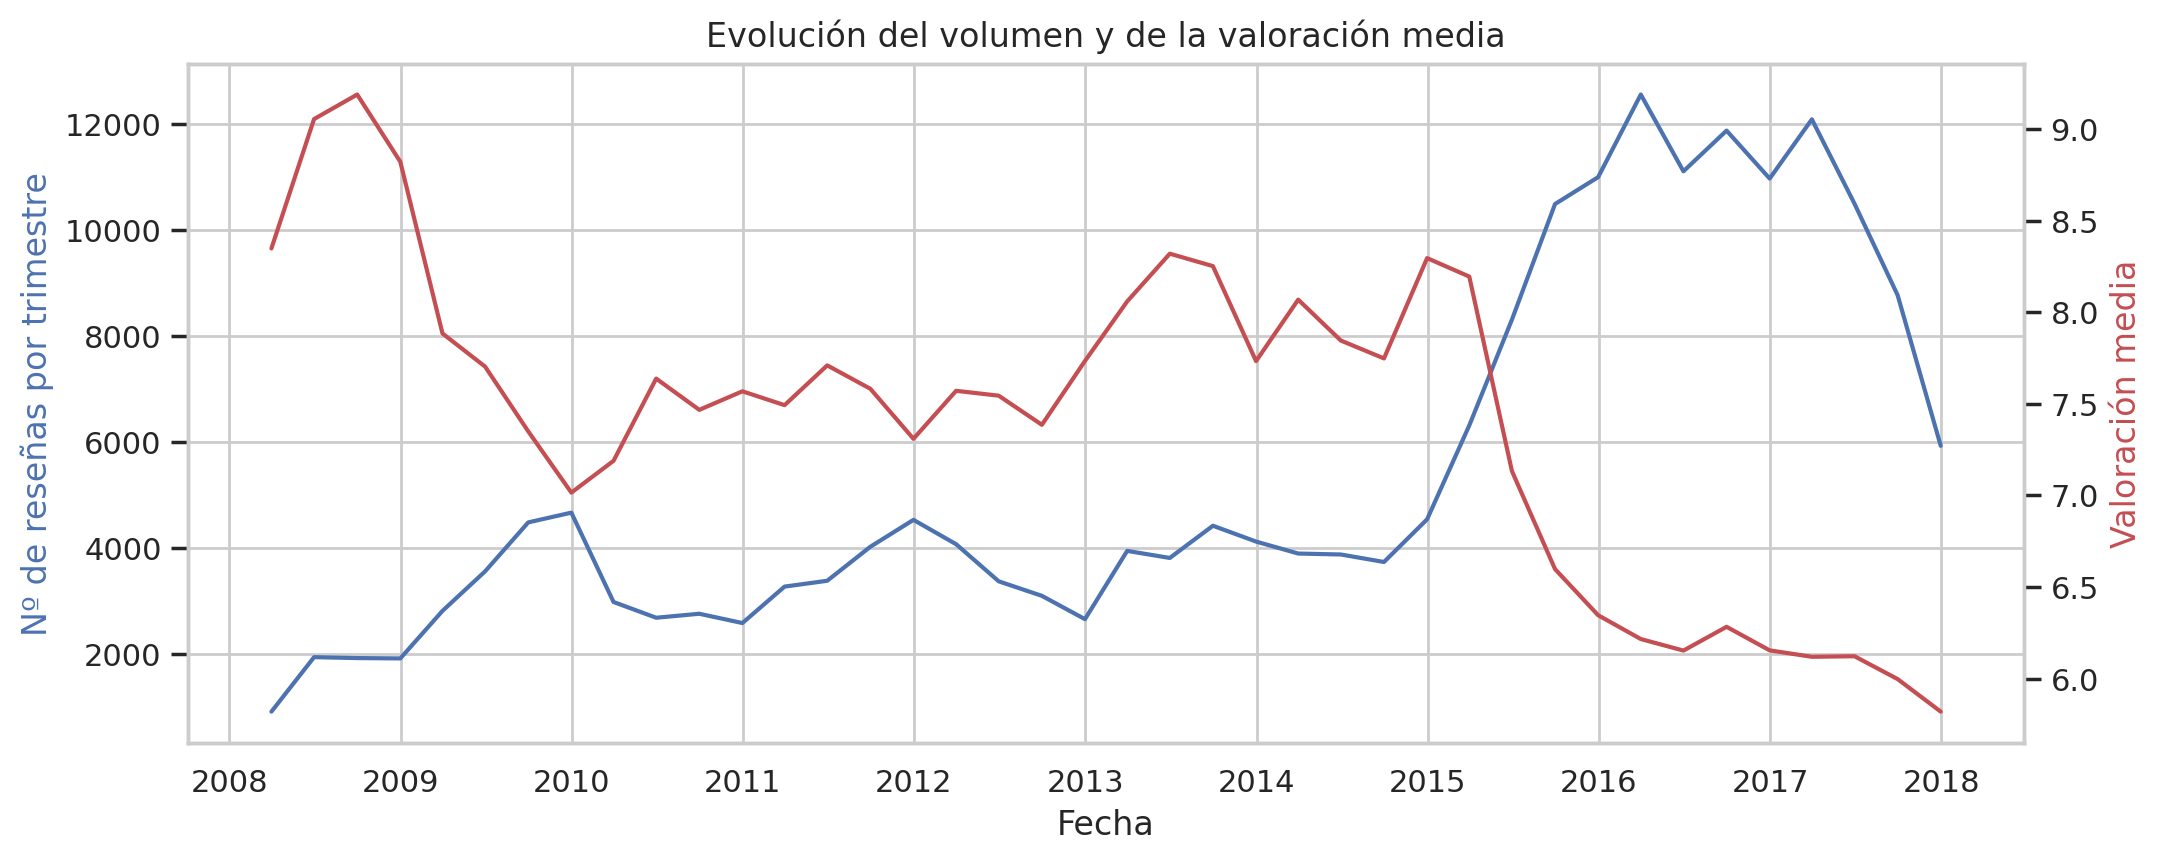
\includegraphics[width=\textwidth]{05_evolucion_temporal}
  \caption{Evolución del volumen de reseñas y de la valoración media por
           trimestre, de 2008 a 2017.}
\end{figure}

\clearpage

% =====================================================================
\section{Resultados detallados}
% =====================================================================

\begin{figure}[htbp]\centering
  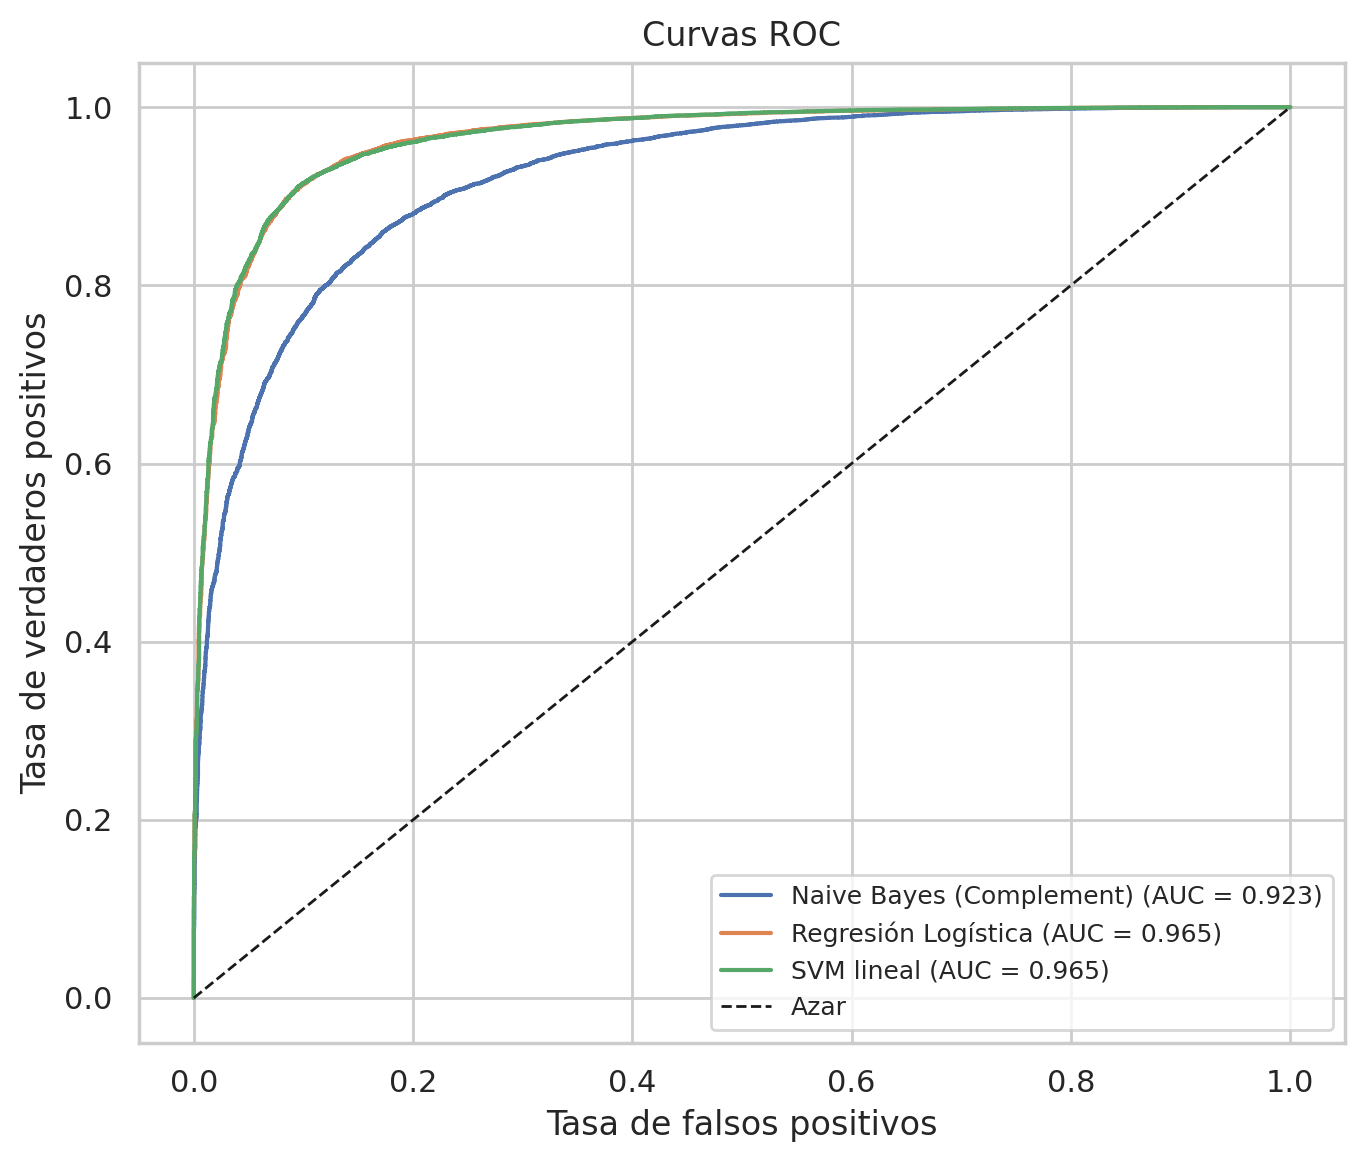
\includegraphics[width=0.72\textwidth]{07_curvas_roc}
  \caption{Curvas ROC de los modelos evaluados.}
\end{figure}

\subsection*{Informe de clasificación por clase}

Complementa la Tabla~4 con el detalle de los dos modelos extremos de la
comparativa.

\vspace{0.2cm}
\begin{center}\small
\begin{tabular}{@{}llcccc@{}}
\toprule
\textbf{Modelo} & \textbf{Clase} & \textbf{Precisión} & \textbf{Recall} & \textbf{F1} & \textbf{Casos} \\ \midrule
SVM lineal          & Negativa & 0,8661 & 0,7972 & 0,8302 & 8.683 \\
                    & Positiva & 0,9379 & 0,9613 & 0,9494 & 27.644 \\ \addlinespace
Random Forest (LSA) & Negativa & 0,6807 & 0,7632 & 0,7196 & 8.683 \\
                    & Positiva & 0,9227 & 0,8876 & 0,9048 & 27.644 \\ \bottomrule
\end{tabular}
\end{center}

\vspace{0.3cm}
El contraste es revelador: sobre la clase positiva ambos modelos son
comparables, pero sobre la negativa —la que importa— Random Forest pierde
19 puntos de precisión. Confirma que la diferencia entre ambos no está en la
capacidad de clasificar en general, sino en detectar la señal minoritaria.

\subsection*{Ficheros de métricas}

\begin{center}\small
\begin{tabular}{@{}ll@{}}
\toprule
\textbf{Fichero} & \textbf{Contenido} \\ \midrule
\texttt{eda\_resumen.json}            & Estadísticos descriptivos y contrastes \\
\texttt{modelado\_resultados.json}    & Métricas de los 5 modelos y coeficientes \\
\texttt{temas\_y\_explicabilidad.json} & Temas NMF, aspectos y casos LIME \\ \bottomrule
\end{tabular}
\end{center}

\end{document}
